%\documentclass{article}
\documentclass[12pt]{report}
\linespread{1.5}

%% Useful packages
\usepackage[a4paper,top=3cm,bottom=3cm,left=3.5cm,right=3cm,marginparwidth=1.75cm]{geometry}
\usepackage{amsmath}
\usepackage{cite}
\usepackage{courier}
\usepackage{caption}
\usepackage{graphicx}
\usepackage[colorinlistoftodos]{todonotes}
\usepackage[colorlinks=true, allcolors=blue]{hyperref}
\usepackage{float}
\usepackage{setspace}
\usepackage{subfigure}
\usepackage{url}
\usepackage{tabularx}
\usepackage[utf8]{inputenc}
\usepackage{mathptmx} %Times Font
\usepackage{mathrsfs}
\usepackage{enumerate}
\usepackage{paralist}
\usepackage{mdwlist}
\usepackage{ulem}
\usepackage{threeparttable}
\usepackage{bm}
\usepackage{listings}
%\usepackage[framed,numbered,autolinebreaks,useliterate]{mcode}
\usepackage{xcolor}
\usepackage{pdfpages}

\usepackage{amsmath}
\DeclareMathOperator*{\argmax}{arg\,max}
\DeclareMathOperator*{\argmin}{arg\,min}

%tikz settings
\usepackage{tikz}
\usetikzlibrary{shapes.geometric}
\usetikzlibrary{arrows.meta,arrows}
\tikzstyle{decision} = [diamond, draw, fill=blue!20, 
text width=6em, text badly centered, node distance=3cm, inner sep=0pt]
\tikzstyle{block} = [rectangle, draw, fill=white, 
text width=9em, text centered, rounded corners, minimum height=4em]
\tikzstyle{block2} = [rectangle, draw, fill=yellow!20, 
text width=9em, text centered, rounded corners, minimum height=4em]
\tikzstyle{line} = [draw, -latex']
\tikzstyle{cloud} = [draw, ellipse,fill=red!20, node distance=3cm,
minimum height=4em]

\newcommand{\tabincell}[2]{\begin{tabular}{@{}#1@{}}#2\end{tabular}}
\newif\ifoutputscaleerror\outputscaleerrorfalse


\begin{document}

%==== FRONT PART====
\begin{titlepage}

\begin{figure}[H]
\centering

\includegraphics[scale=0.8]{Title/logo.eps}
\caption*{}
\label{fig:entropy} 
\end{figure}

\centering

~\\[0.4in]

%\LARGE{\textbf{Place Recognition and Localization for Multi-Robot SLAM}}\\[2in]
{\fontfamily{qhv}\selectfont
	\uppercase{\textbf{\large{Quantitative Trajectory Evaluation Criterion and Long-term Enhancement\\ for Multi-Robot SLAM}\\[2in]
\normalsize	{Liu Xiangyu\\
SCHOOL OF ELECTRICAL AND ELECTRONIC ENGINEERING\\
2019}}}}

\newpage
\end{titlepage}
\begin{titlepage}

\begin{figure}[H]
\centering

\includegraphics[scale=0.8]{Title/logo.eps}
\caption*{}
\label{fig:entropy} 
\end{figure}

\centering
\LARGE{\textbf{Place Recognition and Localization for Multi-Robot SLAM}}\\[2in]



\large{\textbf{Liu Xiangyu}}\\[1in]

\textbf{SCHOOL OF ELECTRICAL AND ELECTRONIC ENGINEERING}

\textbf{MASTER OF SCIENCE IN COMPUTER CONTROL AND AUTOMATION}\\[0.25in]

\textbf{2019}
\newpage
\end{titlepage}

\includepdf[pages={1,2,3}]{Statements/statements.pdf} 
%\begingroup
%\let\cleardoublepage\clearpage
\pagenumbering{roman}
\tableofcontents
%\endgroup

%=== FRONT PART ===
%=== ABSTRCT ===

%\begin{center}
\chapter*{Abstract}
%\end{center}
\addcontentsline{toc}{chapter}{Abstract}

Abstract goes here.\\
Here.\\


\par
\textbf{Keywords:} Dissertation, keywords.

%=== END OF CHAPTER ONE ===

%=== FRONT PART ===
%=== ACKNOWLEDGEMENT ===

%\begin{center}
\chapter*{Acknowledgement}
%\end{center}
\addcontentsline{toc}{chapter}{Acknowledgement}

This dissertation is finished under the guidance of Professor Wang Danwei, in ST Engineering-NTU ROBOTICS ADVANCe LABORATORY in NTU.
I sincerely thank Professor Wang and his PhD students Zhang Jun, Peng Guohao, Yue Yufeng for their patient and careful help during the implementation, experiment and compilation of the dissertation. 
Without their help on providing technical suggestions and possible solutions to the research objectives, and help during the collection of the related datasets, this dissertation project would not go so smoothly within two short semesters.


%=== END OF ACKNOWLEDGEMENT  ===


%%=== FRONT PART ===
%=== ACRONYMS ===

%\begin{center}
\chapter*{Acronyms}
%\end{center}
\addcontentsline{toc}{chapter}{Acronyms}

Acronyms goes here.

%=== END OF ACRONYMS ===

%%=== FRONT PART ===
%=== SYMBOLS ===

%\begin{center}
\chapter*{Symbols}
%\end{center}
\addcontentsline{toc}{chapter}{Symbols}

Symbols goes here.

%=== END OF ACKNOWLEDGEMENT  ===


\listoffigures 
\addcontentsline{toc}{chapter}{Lists of Figures}
\newpage

\listoftables 
\addcontentsline{toc}{chapter}{Lists of Tables}
\newpage


%==== MAIN PART ====
\pagenumbering{arabic}
%=== CHAPTER ONE (1) ===
%=== INTRODUCTION ===

\chapter{Introduction}

\section{Background}

SLAM(Simultaneous localization and mapping) is a key component in mobile autonomous systems. It describes the ability of a vehicle, once placed in an unknown environment, to explore and map that environment, while at the same time estimating its own position in the environment, using only its onboard sensing capabilities.

SLAM systems can be accomplished by both single or multiple robots. Multiple-robot SLAM or MRSLAM, offer several advantages compared to there single robot counterpart, for example:
\begin{itemize}
	\item Robustness to single robot failure,
	\item Quicker exploration of environments in time critical SaR(Search and Rescue) mission.
\end{itemize} 


However, Adapting SLAM technology to multiple-robot scenario brings some new changes as identified by Saeedi et al \cite{saeedi2016multiple}:
\begin{itemize}
	\item Relative Poses of Robots. In multiple-robot SLAM, the map provided by each robot in its own reference coordinates is called the local map. It is difficult task to integrate all of the local maps provided by the other robots to generate a global map of the environment, because the required alignments or transformation matrices, which relate these maps to each other, are in general unknown.
	\item Closing Loops. Loop closure, is defined as identifying a place observed previously but not very recent. Solving this problem for a team of multiple robots requires using all resources of information from individual robots.in Multi-robot SLAM, various events can trigger loop closure, such as direct encounter of the robots or rendezvous and indirect encounter, when the robots see the same area of features in the world.
	\item Communications. Availability of a medium for data sharing among robots is an important requirement in multiple‐robot SLAM. Information between robots can be exchanged via communication channels. The quality of the communication channels is dependent on the environment. For instance, communication issues are a challenging problem for a team of robots in underwater environments, where the environment imposes limitations on the bandwidth and data rate.
\end{itemize}

Because of the limitation of the difficulties mentioned above, the development of multiple-robot SLAM is much slower than single-robot SLAM. Finding a solution to these problem will push the adaption of SLAM technology to a new level.

\begin{figure}[H]
\centering
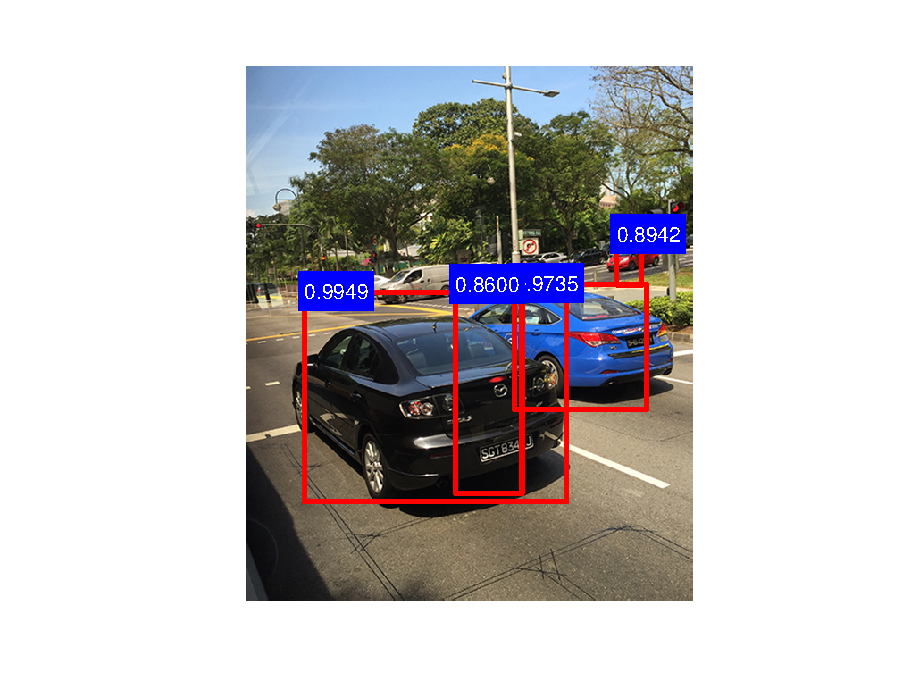
\includegraphics[width=4in]{Chapter1/boundingbox.eps}
\caption{TBD}
\label{fig:boundingboxexample} 
\end{figure}


\section{Motivation and Objectives}

Recently, some solutions for Multi-robot SLAM systems have been proposed.\cite{mcmanus2014shady}




\section{Major contribution of the Dissertation}
\begin{enumerate}[1.]
	\item Evaluation of CORB-SLAM on NTU datasets collected by a cluster of multi ground robots or multi hybrid robots.
	\item Modification of CORB-SLAM to improve its stability and accuracy.
	\item Combination of CORB-SLAM and shade dealing algorithms to enhance its ability to deal with illumination changes.
\end{enumerate}


\section{Organisation of the Dissertation}
This dissertation is organised into several chapters:
\begin{enumerate}[1.]
	\item Chapter 2 briefly outlines the development of visual SLAM technique. Firstly, the classic structure of visual SLAM system is introduced, and the critical algorithms involved are elaborated. The existing solutions are classified into single-robot and multi-robot systems. This chapter also explores prior work in shade dealing algorithms required to implement life-long SLAM.
	
	\item Chapter 3 explains the methodology used in this dissertation to improve the stability and accuracy of CORB-SLAM, and how to combine illumination variance method with CORB-SLAM system to enhance the ability of CORB-SLAM to deal with illumination changes.
	
	\item Chapter 4 shows the results of 
	\begin{inparaenum}[(i)]
		\item the evaluation of CORB-SLAM with NTU datasets.
		\item the evaluation of illumination variant CORB-SLAM with datasets collected under different illumination conditions.
		\end{inparaenum}
		
	\item Chapter 5 analysis the results demonstrated in chapter 4 in detail, discussing the improvement and the disadvantages.
	
	\item Chapter 6 summarizes the work done in this dissertation, and comments on the significance and some potential applications of the proposed solutions.  

\end{enumerate}


%=== END OF CHAPTER ONE ===
\newpage



%=== CHAPTER TWO (2) ===
%=== Literature Review ===

\chapter{Literature Review}

\section{Visual SLAM}

\subsection{Introduction}
Simultaneous Localizaiton and Mapping (SLAM) is a technique to obtain 3D structure of an unknown environment and sensor motion in the environment. After years of development, SLAM-based application have become widely broadened such as computer vision based 3D modeling, augmented reality(AR)-based visualization and self-driving cars. 

In early SLAM algorithms, there exit many different modalities of sensors integrated in SLAM systems, such as rotary encoders, light detection and ranging radar (LiDAR), inertial sensors, GPS and cameras. In recent years, SLAM using cameras only,  specifically referred to as visual SLAM (vSLAM), has been actively discussed because the sensor configuration is simple, low-cost, and contains abundant information. But meanwhile this technique also brings more difficulties than others using integrated sensors\cite{taketomi2017visual}. 

vSLAM algorithms have proposed widely in the field of computer vision, robotics and AR. The low requirement on the modalities of sensors, requiring cameras only, is the major advantage of vSLAM technique, so that it is very suitable for low-cost unmanned vehicles, robots with limited load capacity and power supply like drones, or mobile devices such as camera-mounted tablets or smart phones.

However, the difficulties brought by vSLAM can not be ignored. Instead of obtaining depth and location information directly from LiDAR, GPS or depth camera in integrated SLAM systems, vSLAM technique needs to compute all these information from color or gray images, which reduces stability and accuracy for several estimation steps involved in this process. Also obviously the computational cost are significantly higher. Therefore, the problem of how to improve the performance and reduce computational cost of vSLAM has always been widely concerned.


\subsection{Framework}

The framework of visual SLAM is mainly composed of three modules as follows:
\begin{enumerate}[1.]
	\item Sensor Data Collection
	\item Visual Odometry
	\item Global Map Optimization
	\item Loop Detection
	\item Mapping
\end{enumerate}
 This framework is illustrated in Figure \ref{fig:vslamframe}.

\begin{figure}[!ht]
  \centering
 % \hspace*{-135pt}
  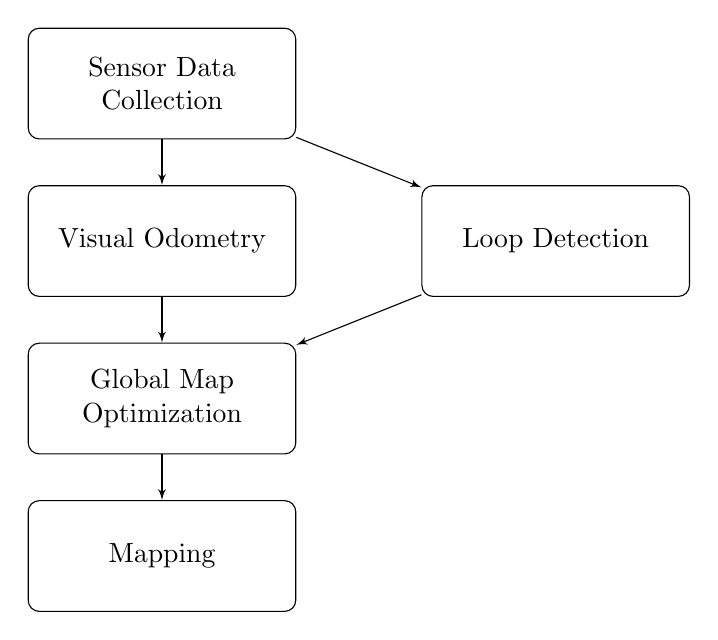
\begin{tikzpicture}[node distance = 2cm, auto]
    % nodes
    \node [block] (init) { Sensor Data Collection};
    \node [block, below of = init] (contact) { Visual Odometry};
    \node [block, below of = contact] (consent) { Global Map Optimization};
    \node [block, below of = consent] (screening) { Mapping};
  \node [block, right of =contact, node distance =5cm](lc){ Loop Detection};
    % edges
    \path [line] (init) -- (contact);
    \path [line] (contact) -- (consent);
    \path [line] (consent) -- (screening);
    \path[line](init)--(lc);
   \path[line](lc)--(consent);
      \end{tikzpicture}
      \caption{Classic structure of Visual SLAM}
      \label{fig:vslamframe}
\end{figure}

Sensor data collection module in visual SLAM systems, is responsible to read and preprocess the image information collected from cameras.

In the module of visual odometry, the reconstrcuted map is tracked in the image to estimate the camera pose of the image with respect to the map. In order to do this, feature tracking or feature matching is executed to obtain 2D-3D correspondences between the image and the map. Then, the camera pose is computed by solving the Perspective-n-point (PnP) problem from the correspondences \cite{klette1998three,nister2007minimal}.

The other module is loop detection, or loop closing, which is a technique to acquire the reference information. In this module, loop closure is detected by matching a current image with previously acquired images. if a closed loop is detected, it means one of the previously observed place is revisited. In this case, the accumulative error can be estimated. The closed loops and the estimated accumulative error will be sent to the next module of global map optimization.

The next module is global map optimization. The reconstructed map includes accumulative estimation error according to the movement distance of the camera. To suppress the accumulative error, the global map optimization is usually performed. In this module, the map is refined according to the consistency of the entire map. When a place is revisited and a closed loop is detected, reference information that represents the accumulative error can be computed. Then global map optimizer can suppress the accumulative error using loop closure from the reference information as a constraint.

Mapping is the last module. In this module, the map is constructed and expanded by computing the 3D structure of the environment according to the information collected and computed in the prior modules.

\subsection{Algorithms}


\section{Visual SLAM Solutions}

\subsection{ORB-SLAM}
\cite{mur2015orb} \cite{mur2017orb}
\begin{figure}[H]
\centering
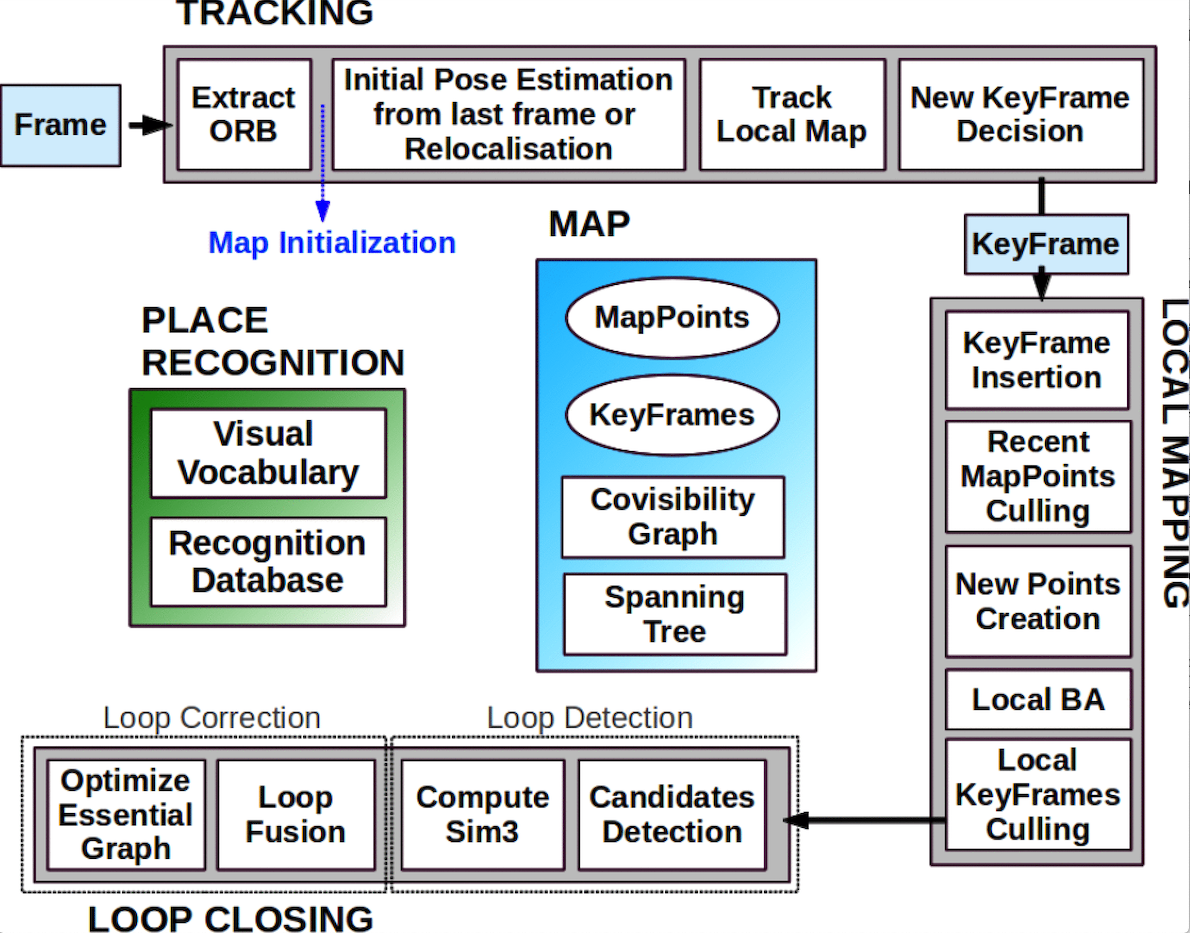
\includegraphics[width=4in]{Chapter2/ORBSLAMOverview.eps}
\caption{ORB-SLAM system overview.}
\label{fig:orbslamoverview} 
\end{figure}

\subsection{CORB-SLAM}
\cite{li2017corb}
\begin{figure}[H]
\centering
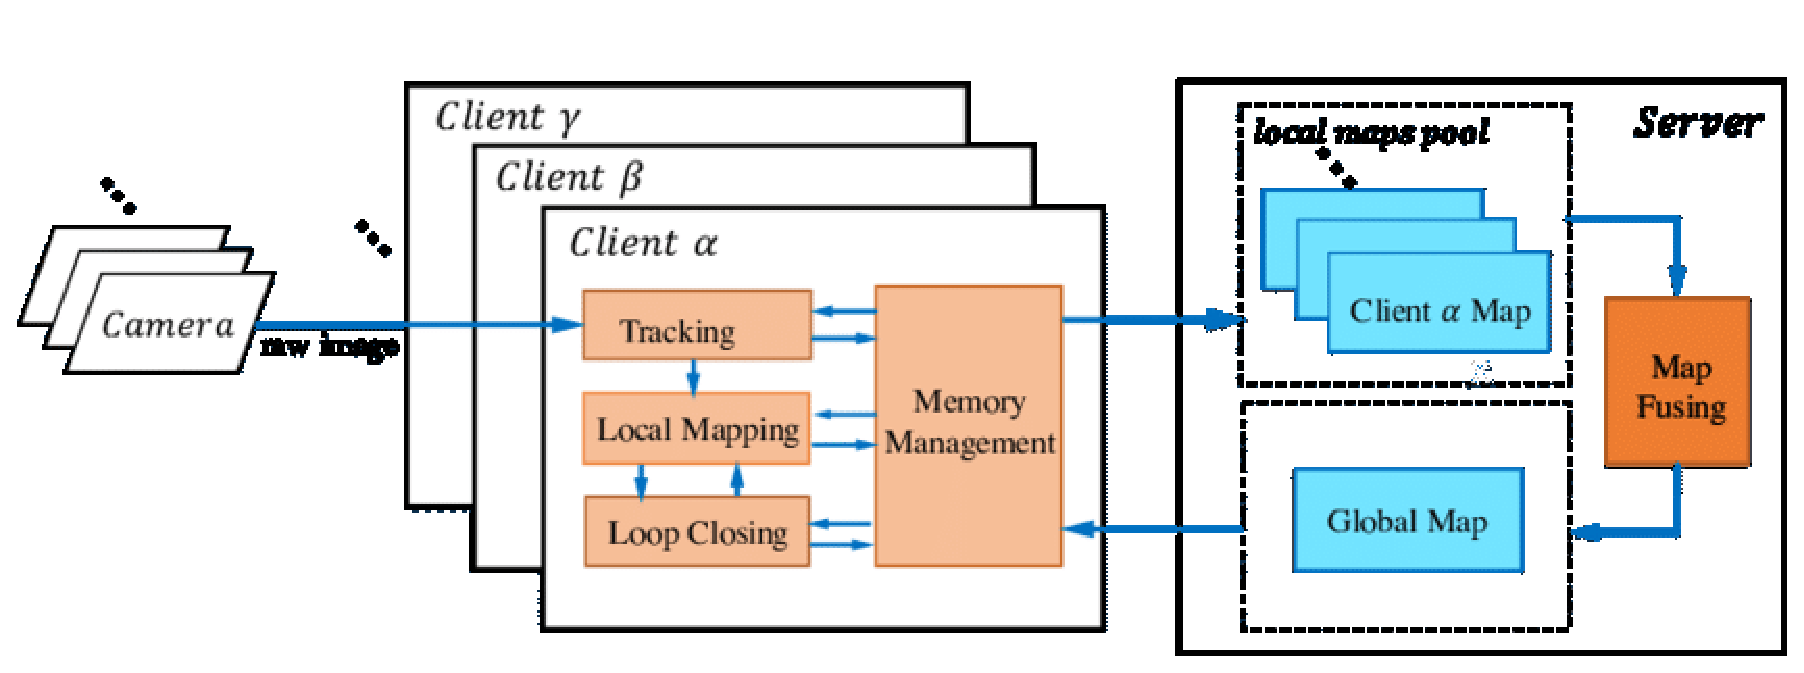
\includegraphics[width=4in]{Chapter2/CORBSLAMOverview.eps}
\caption{The framework of CORB-SLAM system.}
\label{fig:corbslamoverview} 
\end{figure}

\section{Shade Dealing Algorithms}

\subsection{Model-based Approaches}

\subsection{Illumination Variance}
Model-based shade dealing approaches can remove shade more precise, with fewer image details lost, however, obviously their disadvantages limits their application. Model-based approaches requires the type and position of light sources as a prior information to model the illumination patterns, which process has high computational complexity. But vSLAM systems have significant computational cost already, usually deployed on platforms with limited computation capacity, and in most of cases, vSLAM runs in an indoor or outdoor real-world environment with  information of light sources unknown. Therefore,  these two disadvantage determine model-based approaches are not suitable to be combined with vSLAM.

In the case of vSLAM, considering the requirement of low computational complexity and lower image resolution is acceptable, a simpler approach without modeling is preferred. 

Illumination variance approach proposed in \cite{maddern2014illumination}, is a simple method based on only one equation computing illumination variant images.



 \cite{mcmanus2014shady} \cite{arroyo2016openable}
 
 \begin{equation}
 R^{x,E}=
 \end{equation}
 
\begin{equation}
I=\log(R_2)-\alpha\log(R_1)-(1-\alpha)\log(R_3)
\label{eq:iifinal}
\end{equation}

\subsection{Life-Long SLAM}

\begin{figure}[H]
	\centering
	\includegraphics[width=4in]{Chapter2/COISLAMOverview.eps}
	\caption{Block-flow diagram of the combined stereo localisation approach.}
	\label{fig:coislamoverview} 
\end{figure}

%=== END OF CHAPTER TWO ===
\newpage

%=== CHAPTER THREE (3) ===
%=== (Actual work done and contribution, including literature survey) ===

\chapter{Approach (Actual work done and contribution, including literature survey)}

\section{Evaluation of CORBSLAM}

\section{Modification to CORBSLAM}

\section{CORBSLAM with Illumination Variance}




%=== END OF CHAPTER THREE ===
\newpage

%=== CHAPTER FOUR (4) ===
%=== Test and Experiments ===

\chapter{Test and Experiments}

\section{Datasets}

Evaluation are performed in several datasets including KITTI stereo 2015 dataset\cite{Menze2015CVPR},  Oxford RobotCar dataset\cite{maddern20171} and NTU dataset collected in NTU. The listing of used datasets is shown in Table \ref{tbl:datasetsinfo}


\begin{table*}
	\centering
	\caption{Information of datasets used }
	\begin{tabular}{|c|c|c|c|}
		\hline
		Datasets & Settings & Approx Scale & Diversity \\
		\hline
		KITTI &  rural area & $<$ 1 hour & one city, one weather condition, daytime \\
		\hline
		Oxford &  city & 214 hours & one city, multiple weather conditions, daytime \\
		\hline
		NTU &  campus & $<$ 1 hour & one campus (NTU), one weather condition \\
		\hline
	\end{tabular}
	\label{tbl:datasetsinfo}
\end{table*}

\subsection{KITTI Visual Odometry Dataset}

KITTI Visual Odometry 2012 is a part of KITTI Vision Benchmarck Suite, presented in \cite{Geiger2012CVPR,Menze2015CVPR}. KITTI datasets are captured by driving around a mid-size city, in rural areas and on highways. The recording platform is equipped with two high resolution stereo camera systems, capturing color and gray images, a Velodyne HDL-64E LIDAR, and an OXTS RT 3003 localization system which combines GPS, GLONASS, an IMU and RTK correction signals.

KITTI Visual Odometry Evaluation 2012 provides 11 sequences with ground truth trajectories for training, and another 11 sequences without ground truth for evaluation. Example images are shown in Figure \ref{fig:kittiexamples}. 

\begin{figure}[H]
	\centering
	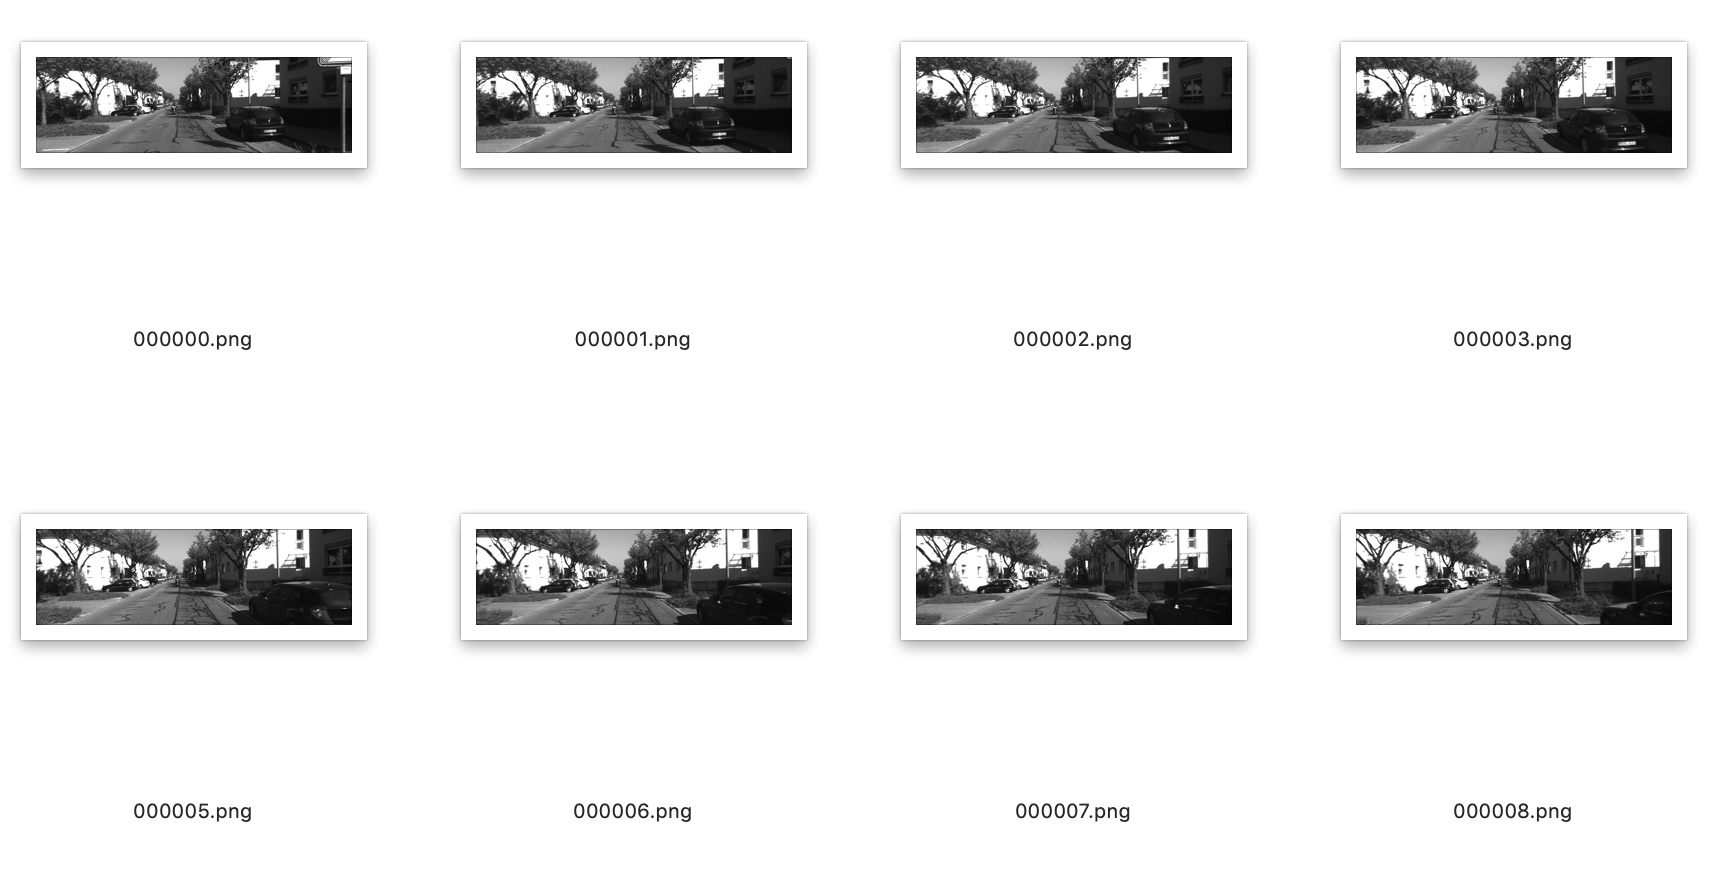
\includegraphics[width=5in]{Chapter4/kittiexamples.eps}
	\caption{Example image in KITTI Visual Odometry 2012 dataset.}
	\label{fig:kittiexamples} 
\end{figure}

\subsection{Oxford RobotCar Dataset}
Oxford RobotCar Dataset is presented by Will Maddern et al. in \cite{maddern20171}, as a challenging dataset for autonomous driving. Collected over the period of May 2014 to December 2015, this datasets recorded images from 6 cameras mounted Nissan LEAF, along with LIDAR, GPS and INS ground truth. Images were recorded under different weather and illumination condition  from 9:00 to 16:00 on average, from May to December. Example images is shown in Figure \ref{fig:robotcarexamples}.

\begin{figure}[H]
	\centering
	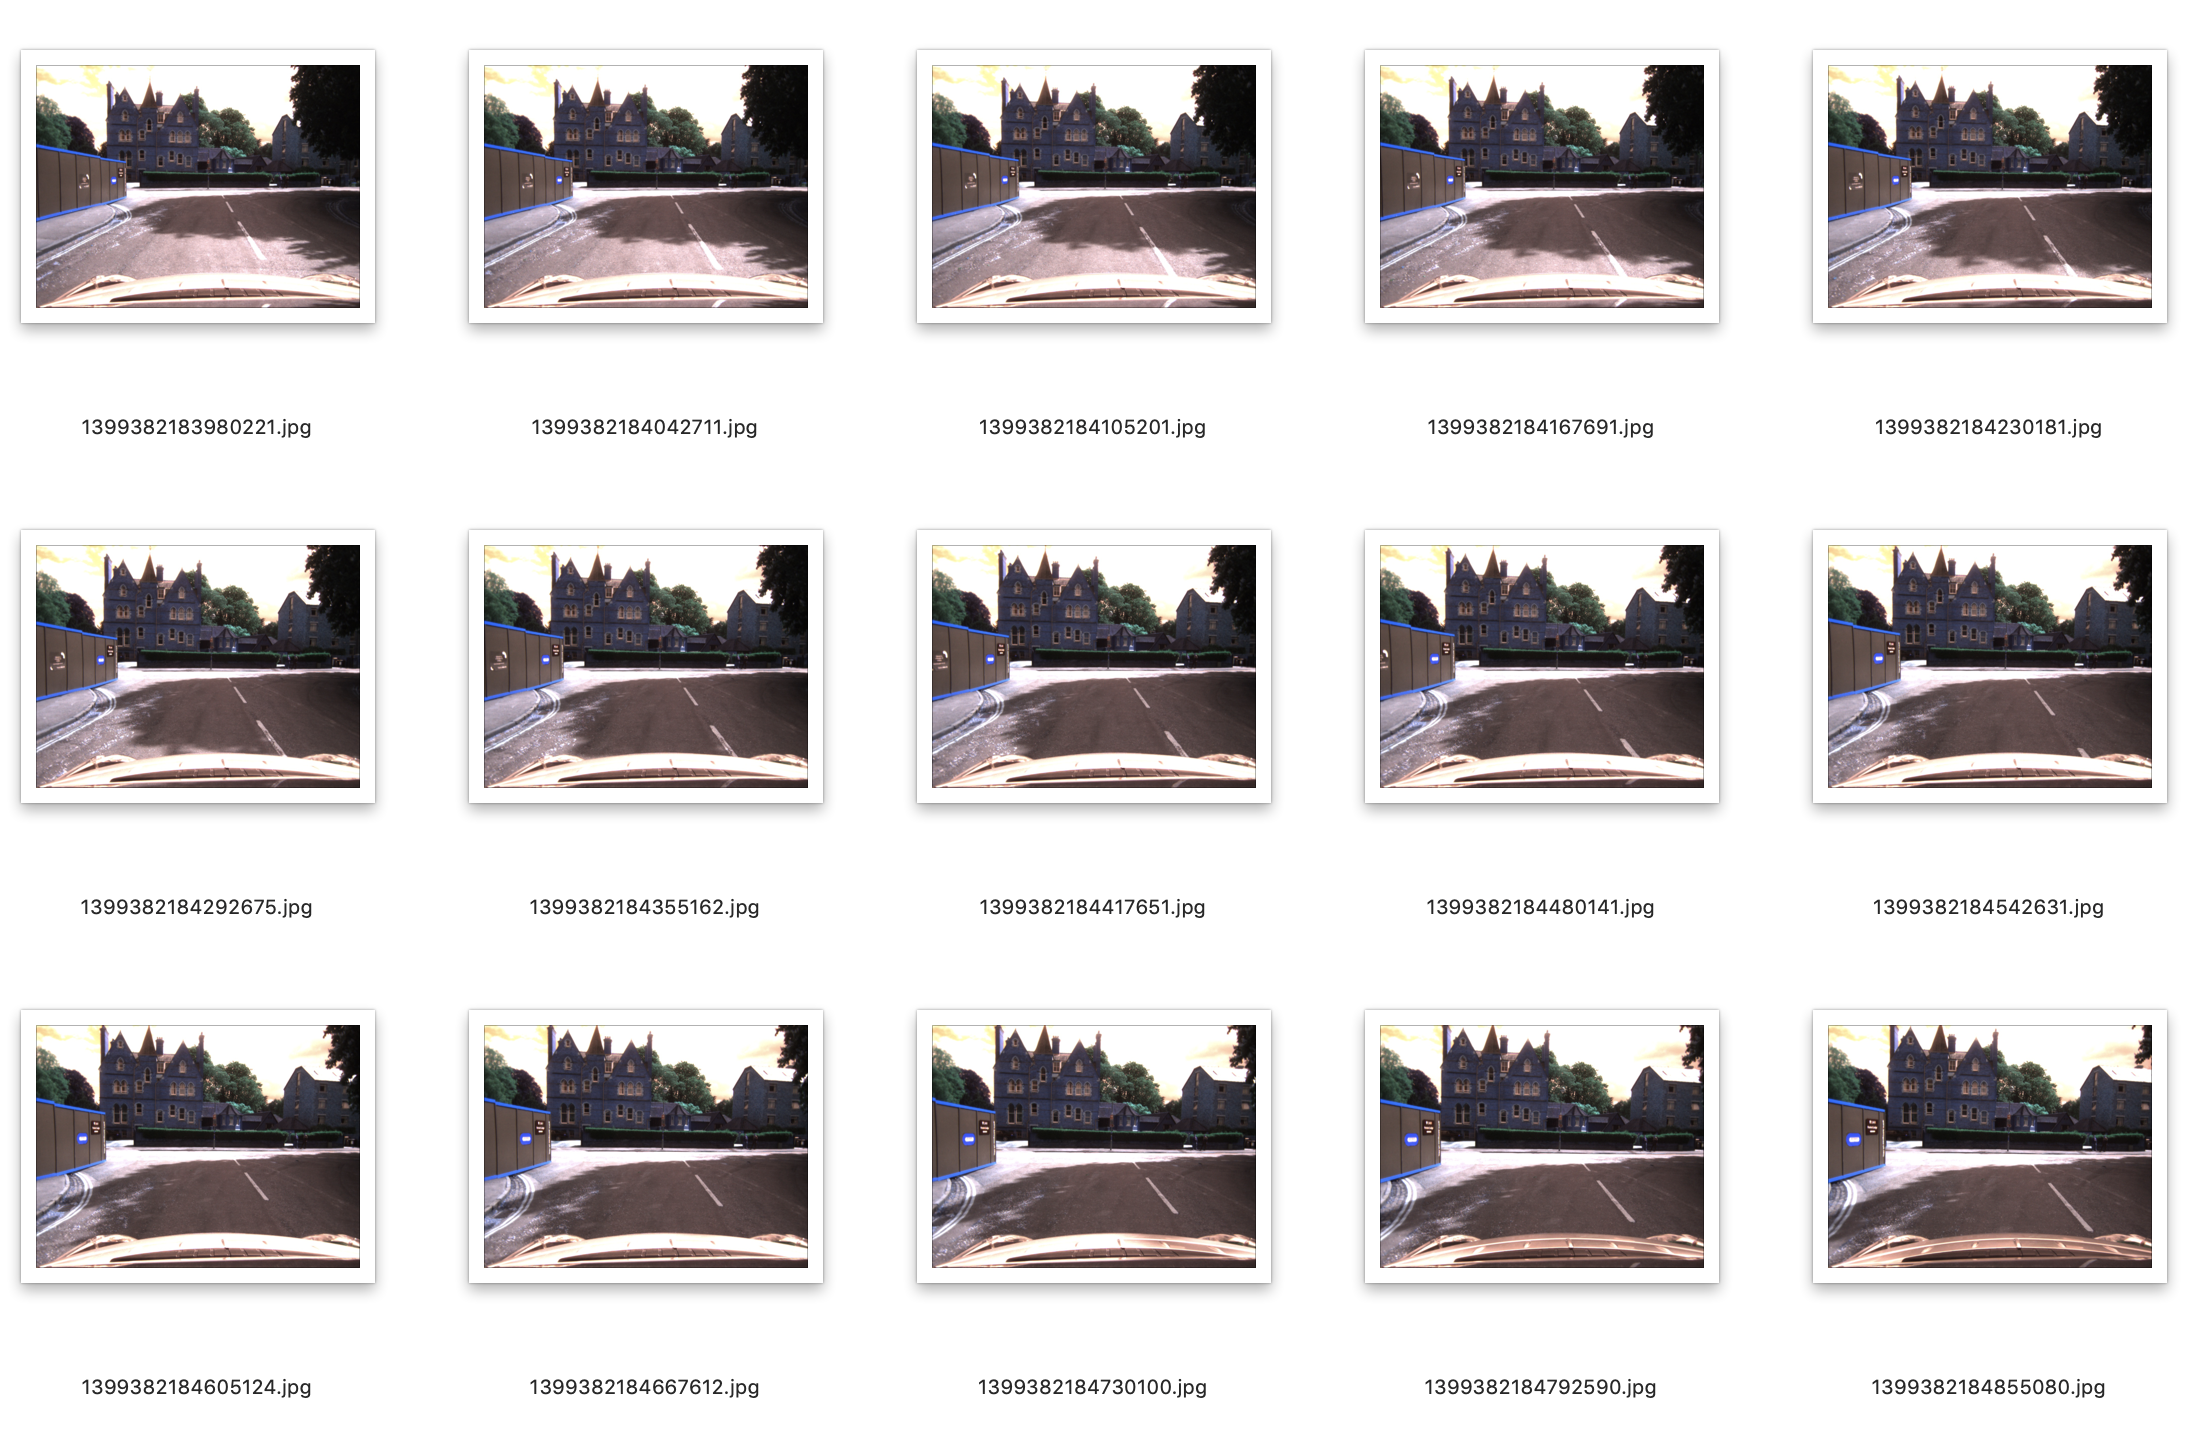
\includegraphics[width=5in]{Chapter4/robotcarexamples.eps}
	\caption{Example image in robotcar dataset.}
	\label{fig:robotcarexamples} 
\end{figure}

The RobotCar platform is a Nissan LEAF equipped with sensors as following \cite{maddern20171}:

\begin{enumerate}
	\item Stereo Camera: Bumblebee XB3 trinocular stereo camera $\times$ 1, 1/3'' Sony ICX445 CCD, 1280$\times$960$\times$3, 16Hz, 3.88mm lens, $66^{\circ}$ HFoV, 12/24cm baseline, global shutter.
	\item Monocular Camera: Grasshopper2 $\times$ 3, 2/3'' ICX285 CCD, 1024$\times$1024, 11.1Hz, 2.67mm fisheye lens, $180^{\circ}$, global shutter.
	\item 2D LIDARL SICK LMS-151 2D LIDAR $\times$ 2, $270^{\circ}$ FoV, 50Hz, 50m range, $0.5^{\circ}$ resolution.
	\item 3D LIDAR: SICK LD-MRS 3D LIDAR $\times$ 1, $85^{\circ}$ HFoC, $3.2^{\circ}$ VFoV, 4 panes, 12.5Hz, 50m range, $0.125^{\circ}$ resolution.
	\item GPS/INS Module: NovAtel SPAN-CPT ALIGN inertial and GPS navigation system $\times$ 1, 6 axis, 50Hz, GPS/GLONASS, dual antenna.
 \end{enumerate}

The RobotCar platform and the sensor locations are demonstrated in Figure \ref{fig:robotcarsensorlocation}.

\begin{figure}[H]
	\centering
	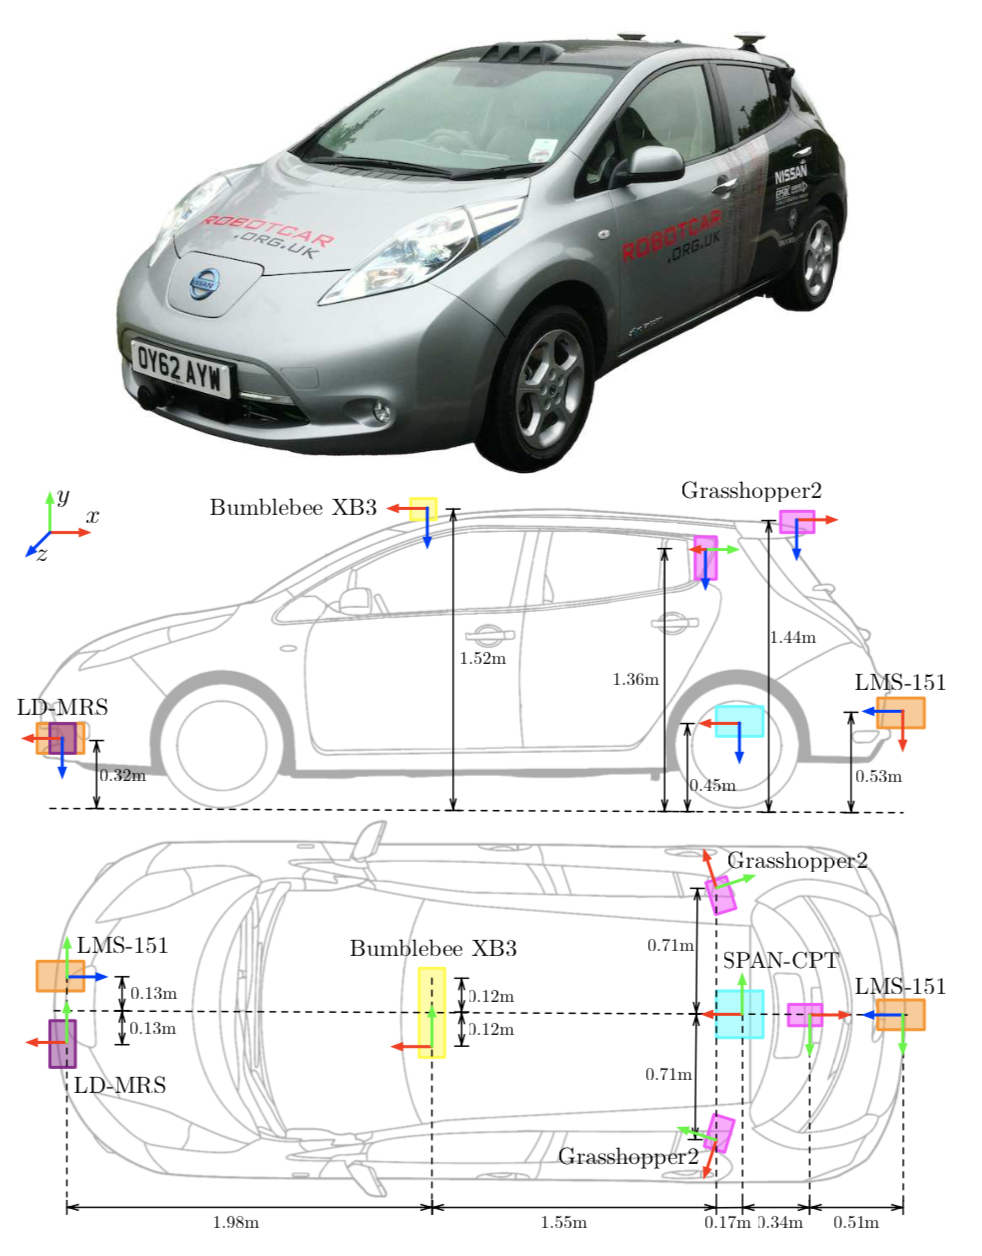
\includegraphics[width=5in]{Chapter4/robotcarsensorlocation.eps}
	\caption{The robotcar platform and sensor location diagram.}
	\label{fig:robotcarsensorlocation} 
\end{figure}

RobotCar dataset is especially suitable to evaluate life-long SLAM systems, since it contains images taken in different hours of daytime under different illumination conditions, and in different seasons. The comparison between image in different illumination conditions and different seasons is shown in Figure \ref{fig:robotcarcomparisonseason}.



\begin{figure}
	\centering
	\subfigure[Image captured in 14:49 07/14/2014.]{
		\begin{minipage}[t]{0.4\linewidth}
			\centering
			\includegraphics[width=2in]{Chapter4/robotcarfeb.eps}
			%\caption{fig1}
		\end{minipage}
	}
	\subfigure[Image captured in 12:32 02/24/2015.]{
		\begin{minipage}[t]{0.4\linewidth}
			\centering
			\includegraphics[width=2in]{Chapter4/robotcardec.eps}
			%\caption{fig2}
		\end{minipage}
	}
	\caption{Comparison of images captured in the same location in different seasons in RobotCar dataset.}
	\label{fig:robotcarcomparisonseason}
\end{figure}
	
\subsection{NTU Dataset}
\label{sec:ntuinfo}
Our NTU dataset is collected by multi hybrid robots consisting of a husky UGV platform and a UAV, recording driving around the carpark in front of School of EEE.

Our UGV platform is a HUSKY Clearpath robot, equipped with a ZED stereo camera $\times$ 1, 672$\times$376, $87^{\circ}$ HFoV, $56^{\circ}$ VFoV. The picture of the platform and example images are shown in Figure \ref{fig:ntuugvplatform} and \ref{fig:ntuexamples}.

The UAV platform is assembled with: PIXRACER V1.0 AUTOPILOT Controller Module, DJI E Series 620S Motor Package, a uBLOXNEO-M8N GPS Module and a monocular camera mounted at a depression angle of 20 degree. The overview picture of the UAV is shown in Figure \ref{fig:ntuuavplatform}

The dataset provides 4 rosbag files. 3 of them are recorded by UGV, while the other one is recorded by UAV. The basic information of 4 rosbags are listed in Table \ref{tbl:ntubagsinfo}. And the ground truth trajectories are shown in Figure \ref{fig:ntugt}.

\begin{figure}
	\centering
	\subfigure[Ground truth trajectory of Bag.0.]{
		\begin{minipage}[t]{0.4\linewidth}
			\centering
			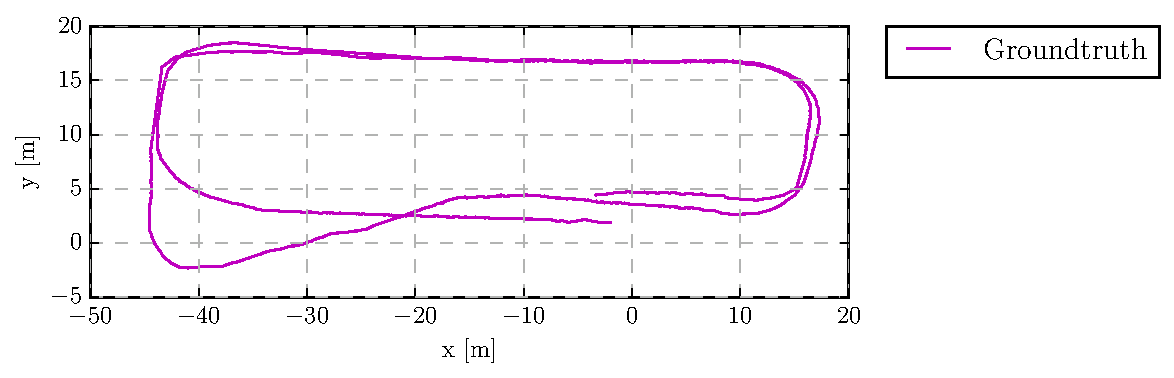
\includegraphics[width=2in]{Chapter4/NTU/0446/trajectory_top_gt_sim3_-1.pdf}
			%\caption{fig1}
		\end{minipage}
	}
	\subfigure[Ground truth trajectory of Bag.1.]{
		\begin{minipage}[t]{0.4\linewidth}
			\centering
			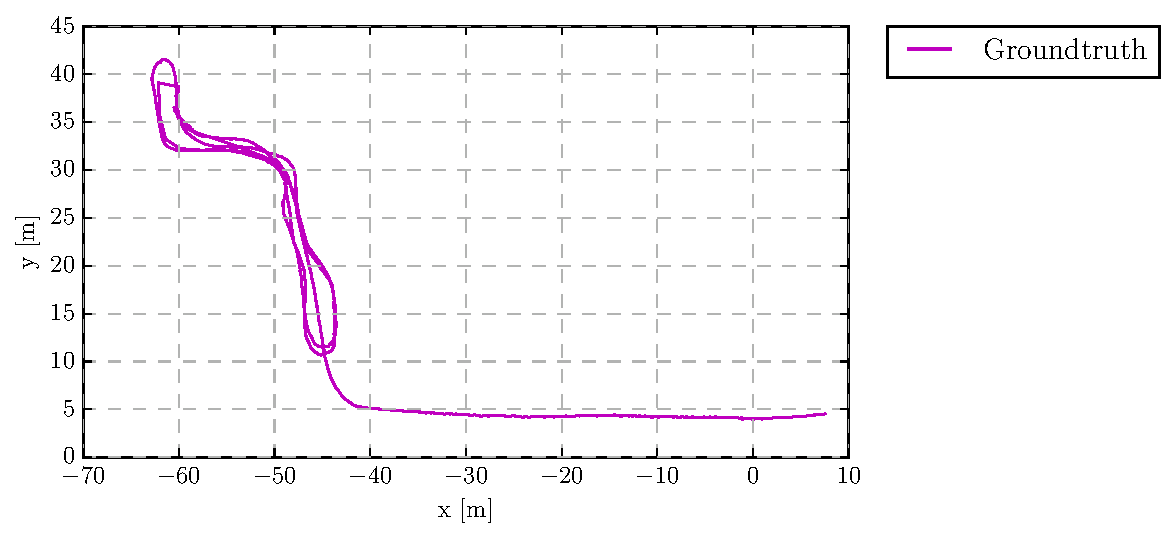
\includegraphics[width=2in]{Chapter4/NTU/0454/trajectory_top_gt_sim3_-1.pdf}
			%\caption{fig2}
		\end{minipage}
	}
	\vfill
		\subfigure[Ground truth trajectory of Bag.2.]{
		\begin{minipage}[t]{0.4\linewidth}
			\centering
			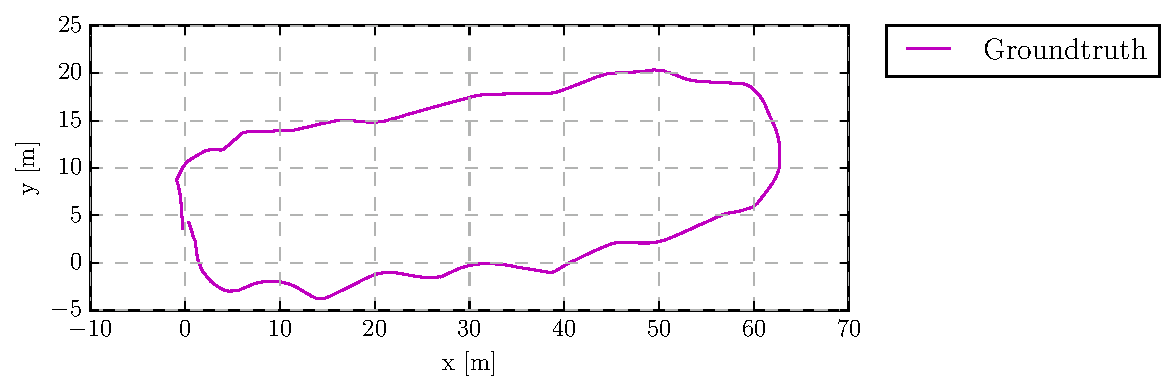
\includegraphics[width=2in]{Chapter4/NTU/UGV/plots/trajectory_top_gt_sim3_-1.pdf}
			%\caption{fig1}
		\end{minipage}
	}
	\subfigure[Ground truth trajectory of Bag.3.]{
		\begin{minipage}[t]{0.4\linewidth}
			\centering
			
\includegraphics[width=2in]{thereisafigure.eps}
			%\caption{fig2}
		\end{minipage}
	}
	\caption{Comparison of images captured in the same location in different seasons in RobotCar dataset.}
	\label{fig:ntugt}
\end{figure}

\begin{table*}
	\centering
	\caption{Main characteristics of the rosbags in NTU Dataset used in the experiment.}
	\begin{tabular}{|c|c|c|c|c|}
		\hline
		Bag No. & Data(M/D/Y)  & Platform & Height(m) & Dep. Angle  \\
		\hline
		0&10/27/2018& UGV & $\approx 0.7m$ & $0^\circ$ \\
		\hline
		1&10/27/2018& UGV & $\approx 0.7m$ & $0^\circ$ \\
		\hline
		2&03/08/2019& UGV & $\approx 0.7m$ & $0^\circ$ \\
		\hline
		3&03/08/2019& UAV & $\approx 2m$ & $20^\circ$ \\
		\hline
	\end{tabular}
	\label{tbl:ntubagsinfo}
\end{table*}

\begin{figure}[H]
	\centering
	\includegraphics[width=5in]{Chapter4/ntuhuskytugv.eps}
	\caption{Overview picture of NTU Husky platform.}
	\label{fig:ntuugvplatform} 
\end{figure}

\begin{figure}[H]
	\centering
	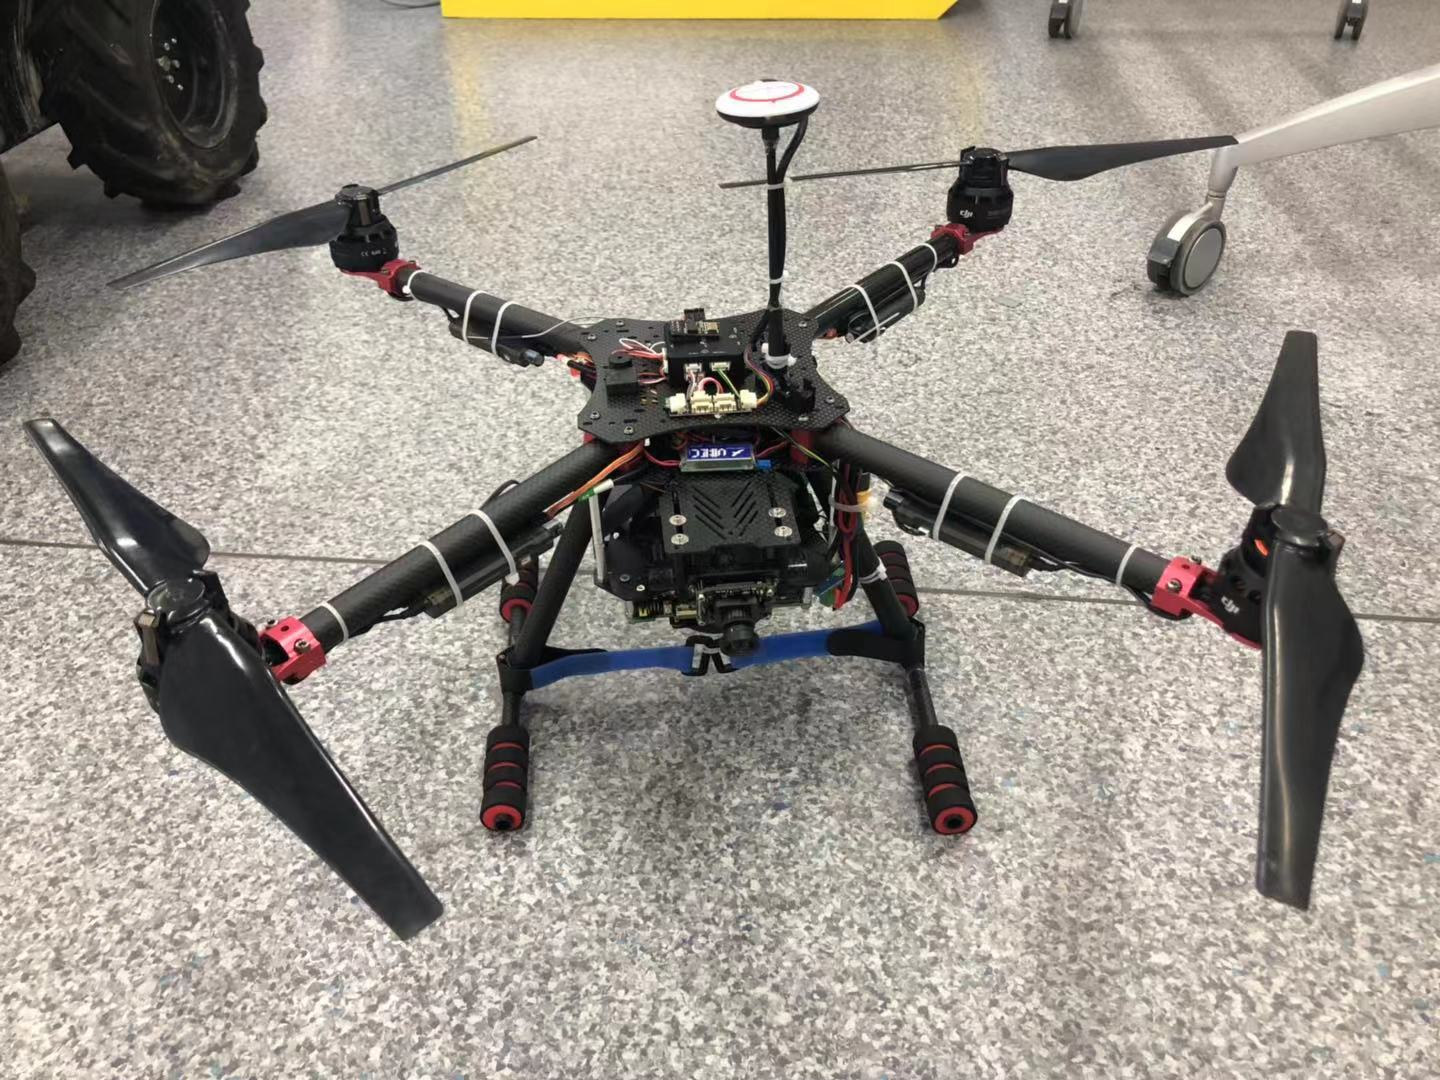
\includegraphics[width=5in]{Chapter4/ntuuav0.eps}
	\caption{Overview picture of NTU Husky platform.}
	\label{fig:ntuuavplatform} 
\end{figure}

\begin{figure}[H]
	\centering
	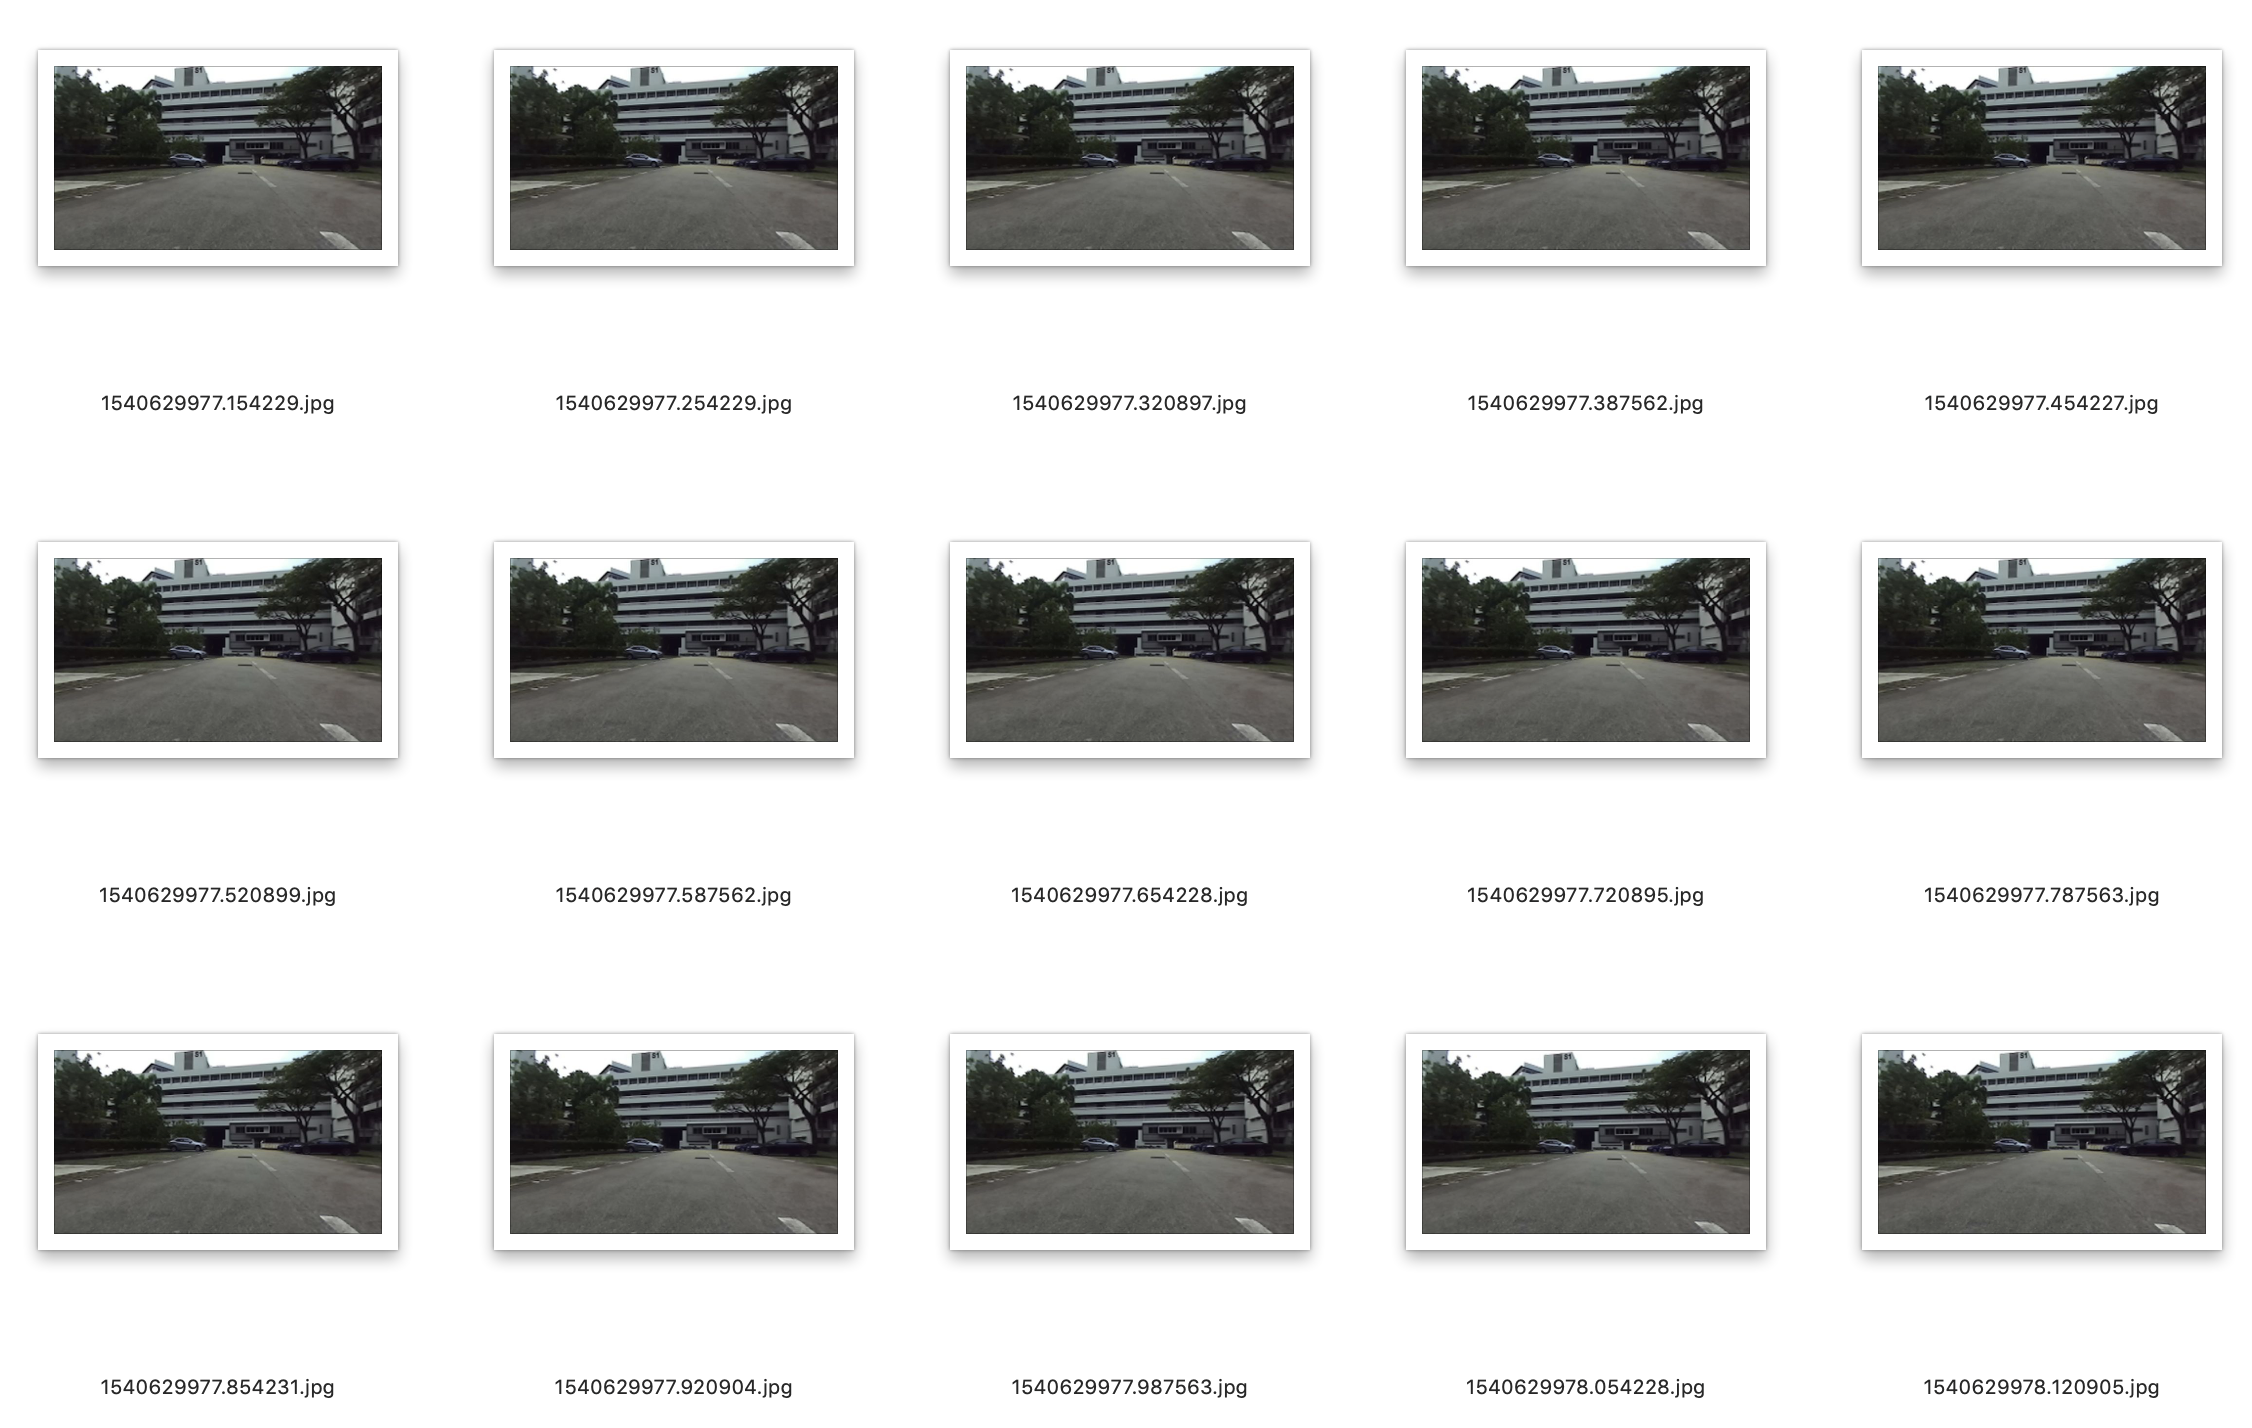
\includegraphics[width=5in]{Chapter4/ntuexamples.eps}
	\caption{Example images of NTU dataset.}
	\label{fig:ntuexamples} 
\end{figure}

\section{Evaluation of CORBSLAM}
\subsection{Evaluation on multi ground robots}

\subsubsection{KITTI Datasets}
\label{sec:kittievaluate}
In order to evaluate CORB-SLAM system, sequence 00 is utilized and separated into two sub sequences with proper length of overlap. The following separating method is employed: We assume the time period of a KITTI sequence if $Seq.0[0,t]$. Then the sequence is separated into two sub sequences $Seq.01[0,\frac{t}{2}+\delta{t}]$ and $Seq.02[\frac{t}{2},t]$ as the assumed input of two client robots. 

Therefore, in this case, Sequence 00 containing $f=4541frames$ and covering a total distance of $s=1856m$ is separated into two partial sequences: Seq.0$[0, \frac{2}{3}f]$ and Seq.1$[\frac{1}{3}f, f]$, both containing  $\frac{2}{3}f\approx{3027frames}$ and covering distances of $\frac{2}{3}s\approx{1237m}$ (a rough estimate since distances between each pair of frames are not equal). 

The ground truth information of Seq.0, Seq.1 and the complete ground truth trajectory of Sequence 00 are shown for reference in Figure \ref{fig:kittigt}. And Figure \ref{fig:kittiresults} demonstrates mapping results of each partial sequence and the map fusion results of the server. Four charts in Figure \ref{fig:kittiquanresult} contains quantitative evaluation results, with corresponding numeric results shown in Table \ref{tbl:ntuquanresult}.

Because the two partial sequences are extracted from Sequence 00, so the completed mapping results of CORB-SLAM client on Sequence 00 can be provided as a comparison by Figure \ref{fig:kittientirequanresult}, \ref{fig:kitticlientmapping} and Table \ref{tbl:kitticlientquanresult} in the same format as above. Results are further discussed in Section \ref{sec:disussmultiground}.

\begin{figure}
	\centering
	\subfigure[Ground truth trajectory of Seq.0.]{
		\begin{minipage}[t]{0.4\linewidth}
			\centering
			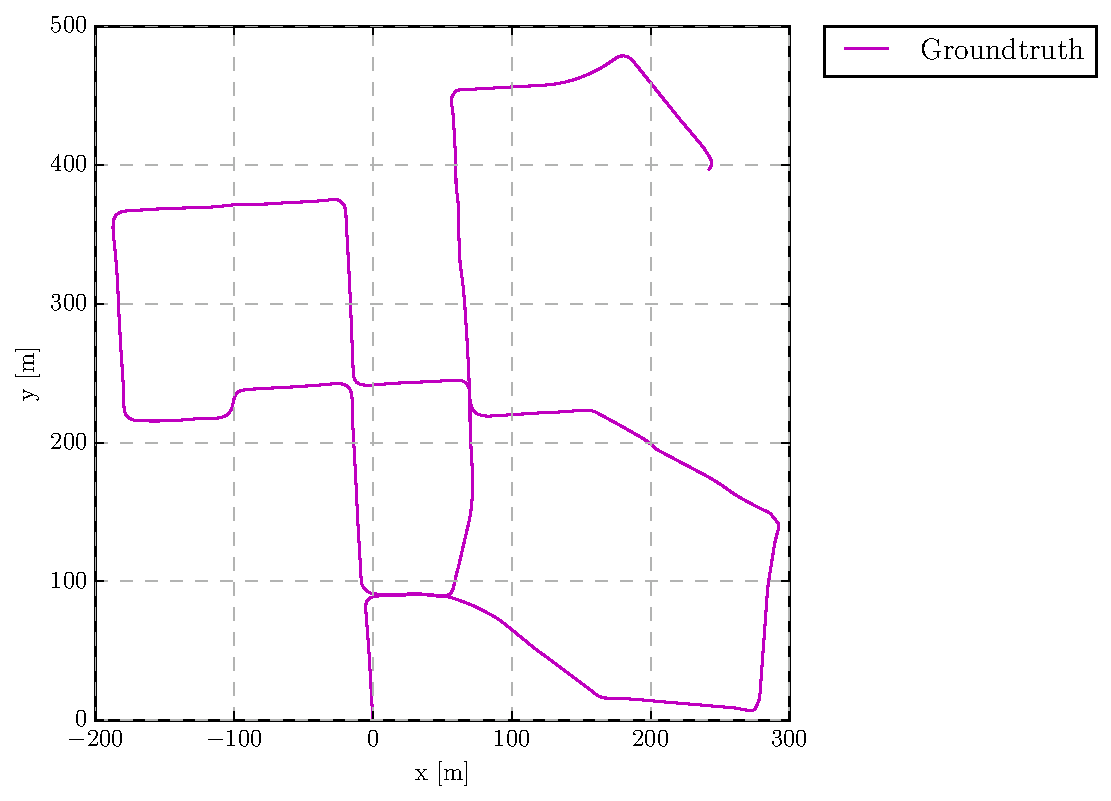
\includegraphics[width=2in]{Chapter4/KITTI/00server/32/plots/trajectory_side_gt_sim3_-1.pdf}
			%\caption{fig1}
		\end{minipage}
	}
	\subfigure[Ground truth trajectory of Seq.1.]{
		\begin{minipage}[t]{0.4\linewidth}
			\centering
			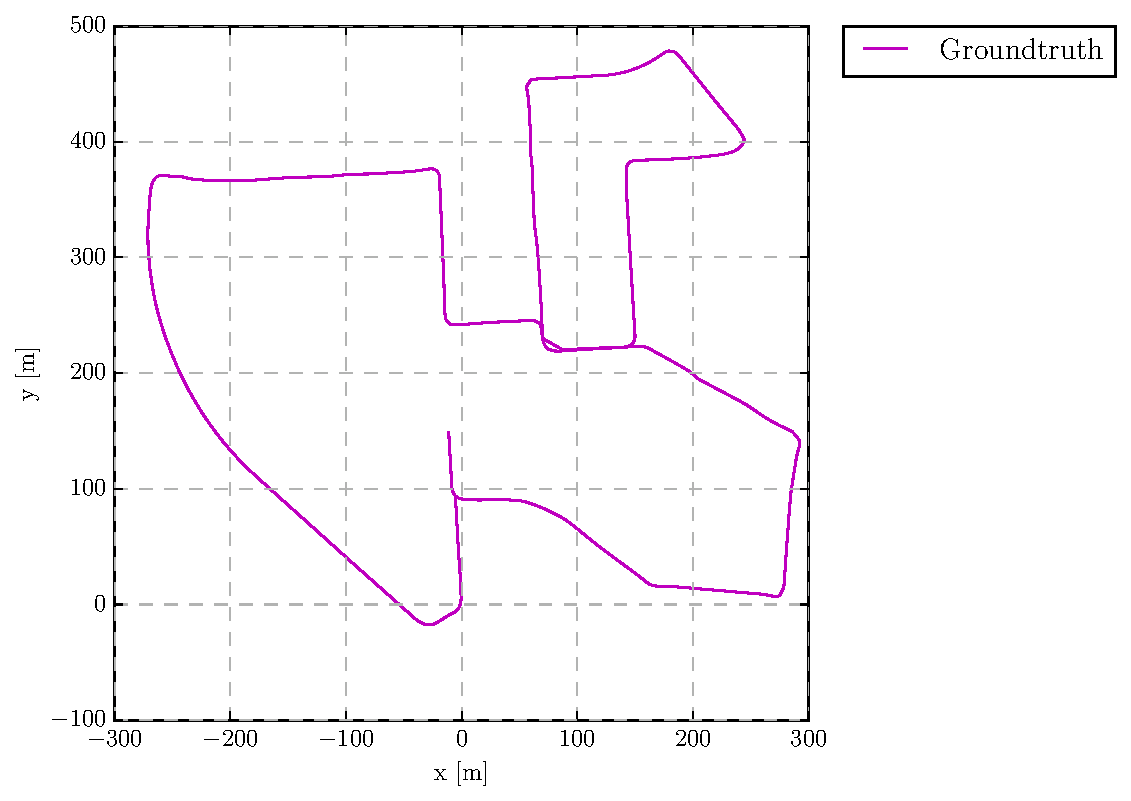
\includegraphics[width=2in]{Chapter4/KITTI/00server/33/plots/trajectory_side_gt_sim3_-1.pdf}
			%\caption{fig2}
		\end{minipage}
	}
	\vfill
	\subfigure[Ground truth trajectory of complete Sequence 00.]{
		\begin{minipage}[t]{\linewidth}
			\centering
			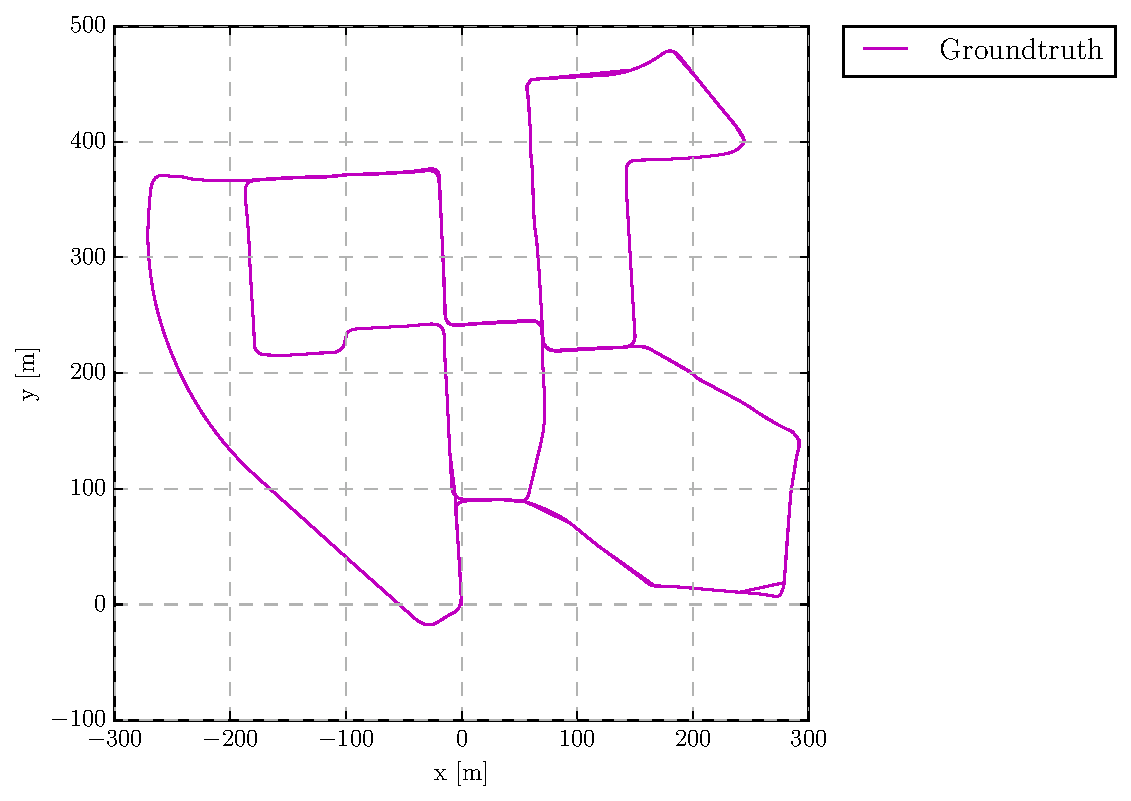
\includegraphics[width=5in]{Chapter4/KITTI/00server/plots/trajectory_side_gt_sim3_-1.pdf}
			%\caption{fig1}
		\end{minipage}
	}
	\caption{Ground truth trajectory of partial and complete sequences of KITTI Datasets.}
	\label{fig:kittigt}
\end{figure}

\begin{figure}
	\centering
	\subfigure[Relative translation error.]{
		\begin{minipage}[t]{0.4\linewidth}
			\centering
			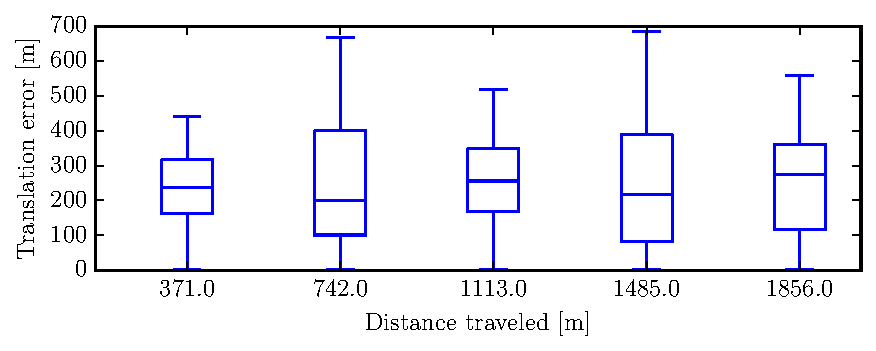
\includegraphics[width=2in]{Chapter4/KITTI/00/gps/plots/rel_translation_error.pdf}
			%\caption{fig1}
		\end{minipage}
	}
	\subfigure[Relative translation error by percent.]{
		\begin{minipage}[t]{0.4\linewidth}
			\centering
			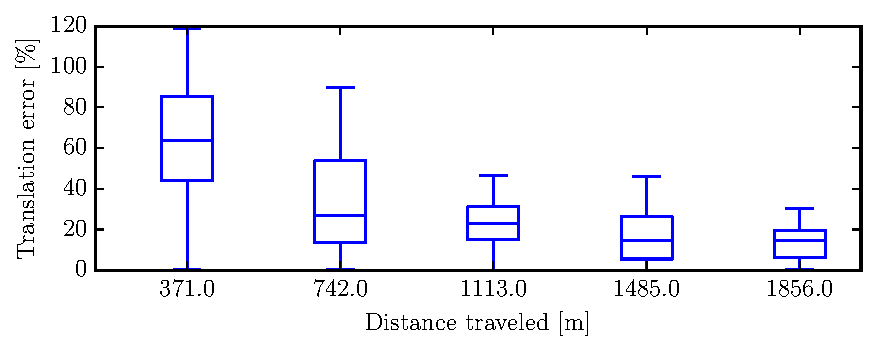
\includegraphics[width=2in]{Chapter4/KITTI/00/gps/plots/rel_translation_error_perc.pdf}
			%\caption{fig2}
		\end{minipage}
	}
	\vfill
	\subfigure[Relative yaw error.]{
		\begin{minipage}[t]{0.4\linewidth}
			\centering
			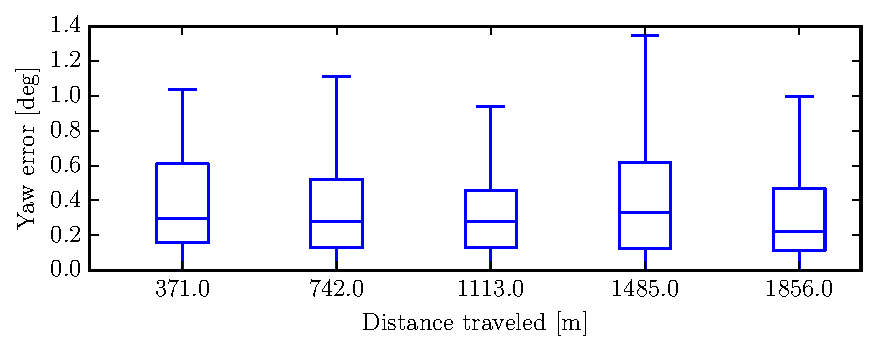
\includegraphics[width=2in]{Chapter4/KITTI/00/gps/plots/rel_yaw_error.pdf}
			%\caption{fig1}
		\end{minipage}
	}
	\subfigure[Scale error.]{
		\begin{minipage}[t]{0.4\linewidth}
			\centering
			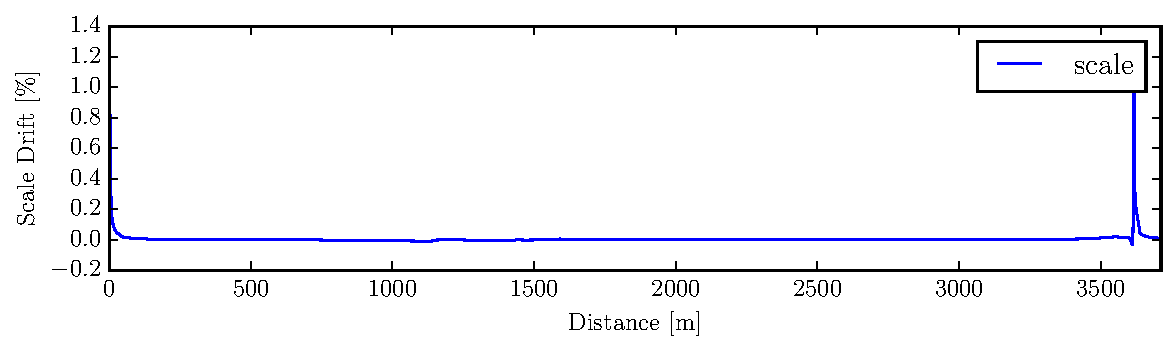
\includegraphics[width=2in]{Chapter4/KITTI/00/gps/plots/scale_error_sim3_-1.pdf}
			%\caption{fig2}
		\end{minipage}
	}
	\caption{Quantitative evaluation results of CORB-SLAM client mapping the entire KITTI Sequence 00.}
	\label{fig:kittientirequanresult}
\end{figure}

\begin{table*}
	\centering
	\caption{Quantitative results of mapping unseparated Sequence 00.}
	\begin{threeparttable}
		\begin{tabular}{|c|c|c|c|c|}
			\hline
			Distance(m)\tnote{1} & Rel. Trans.(m)\tnote{2}  & Rel. Trans.($\%$)\tnote{3} & Rel. Yaw(deg)\tnote{4} & Scale Err.($\%$)\tnote{5}  \\
			\hline
			371& 229.69 & 61.91 & 0.37 & - \\
			\hline
			742&260.10& 35.05 & 0.37 & - \\
			\hline
			1113&260.20& 23.38 & 0.31 & - \\
			\hline
			1485&240.93& 16.22 & 0.40 & - \\
			\hline
			1856&255.16& 13.74 & 0.32 & - \\
			\hline
			-&-&- & - &  0.05\\
			\hline
		\end{tabular}
		\begin{tablenotes}
			\footnotesize
			\item[1] Distance in meter traveled before each time of statistics. 
			\item[2] Mean relative translation error in meter.
			\item[3] Mean relative translation error in percent.
			\item[4] Mean relative yaw error in degree.
			\item[5] Median scale error in percent.
		\end{tablenotes}
	\end{threeparttable}
	\label{tbl:kitticlientquanresult}
\end{table*}

\begin{figure}[H]
	\centering
	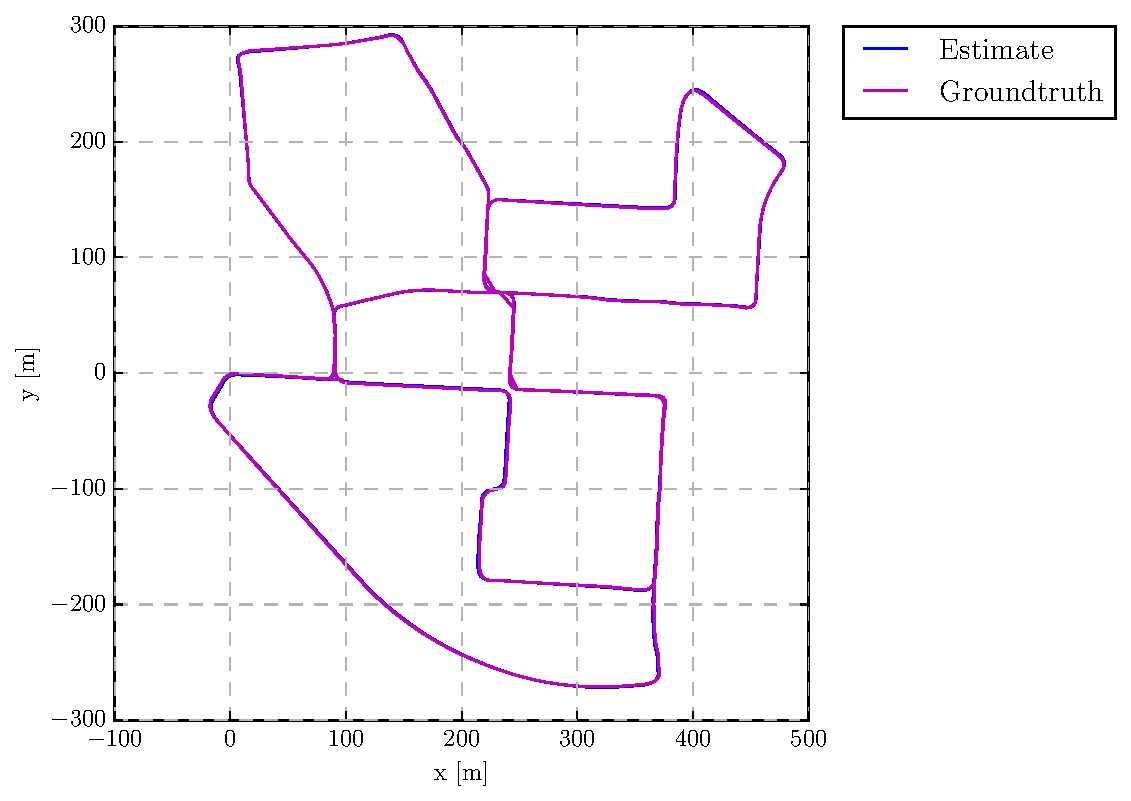
\includegraphics[width=5in]{Chapter4/KITTI/00/gps/plots/trajectory_side_sim3_-1.pdf}
	\caption{Mapping results of the entire sequence without partial sequence.}
	\label{fig:kitticlientmapping} 
\end{figure}

\begin{figure}
	\centering
	\subfigure[Mapping result of Seq.0 compared with ground truth.]{
		\begin{minipage}[t]{0.4\linewidth}
			\centering
			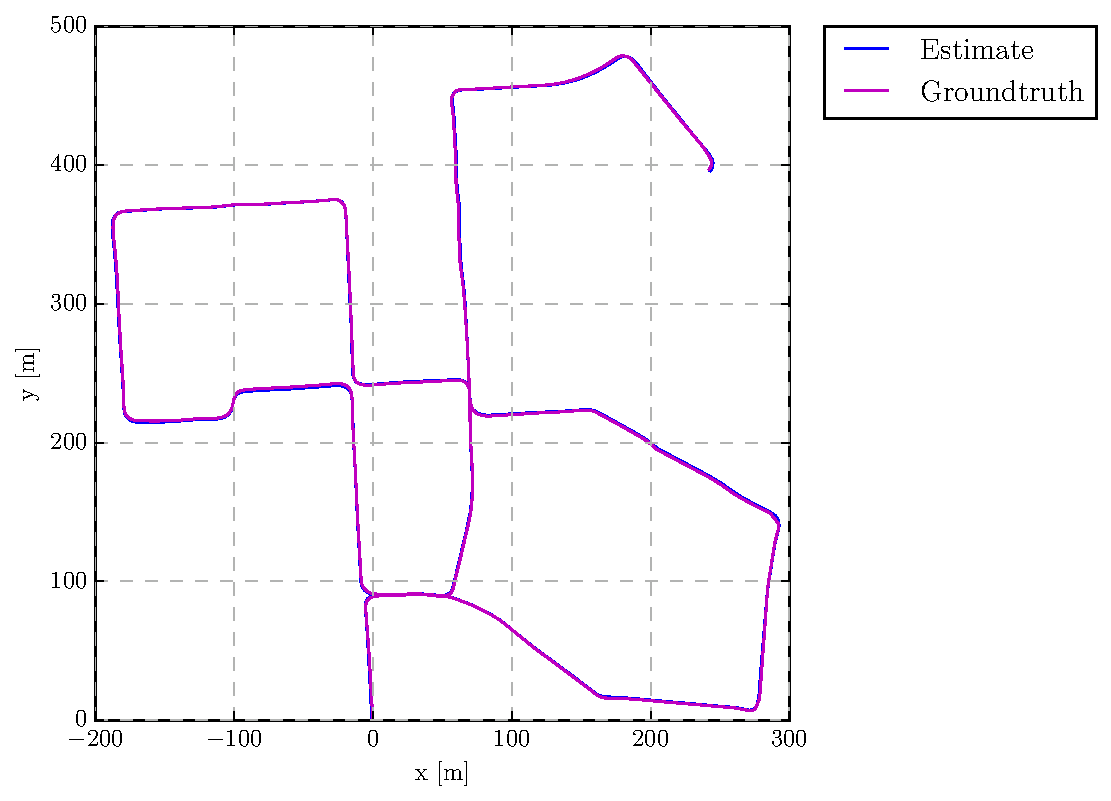
\includegraphics[width=2in]{Chapter4/KITTI/00server/32/plots/trajectory_side_sim3_-1.pdf}
			%\caption{fig1}
		\end{minipage}
	}
	\subfigure[Mapping result of Seq.1 compared with ground truth.]{
		\begin{minipage}[t]{0.4\linewidth}
			\centering
			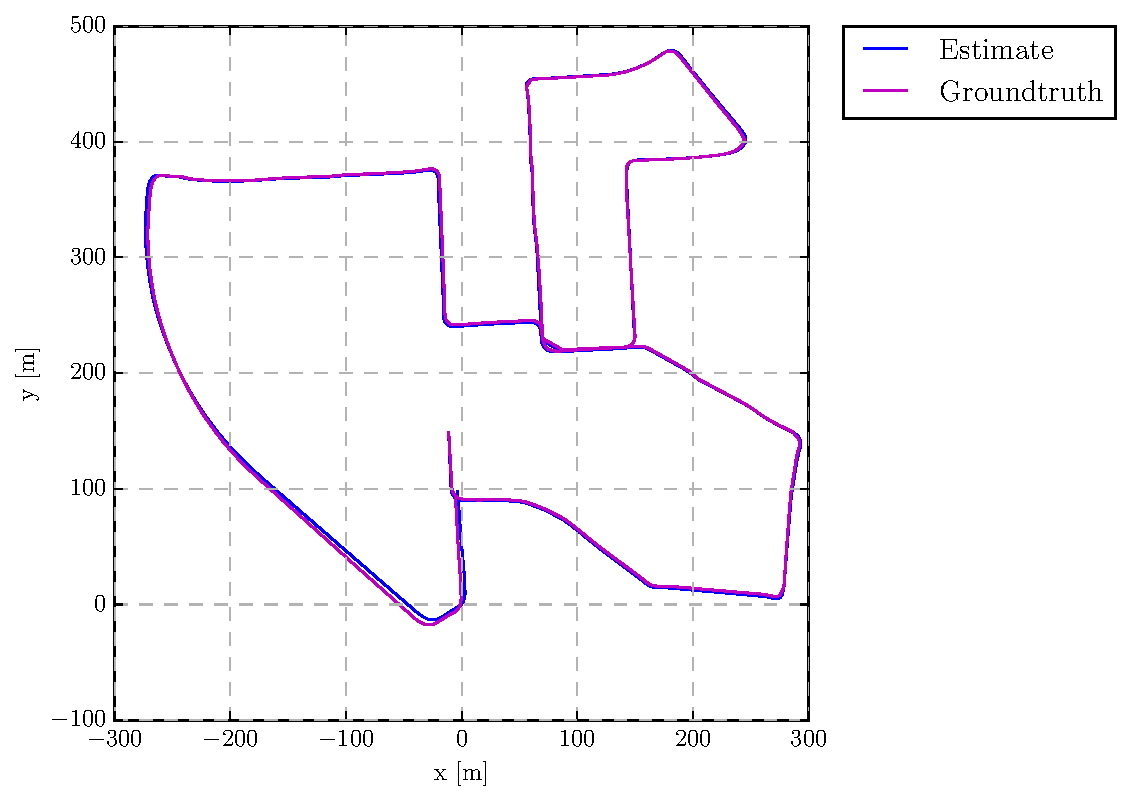
\includegraphics[width=2in]{Chapter4/KITTI/00server/33/plots/trajectory_side_sim3_-1.pdf}
			%\caption{fig2}
		\end{minipage}
	}
	\vfill
	\subfigure[Map Fusion results of Seq.0 and Seq.1 compared with ground truth.]{
		\begin{minipage}[t]{\linewidth}
			\centering
			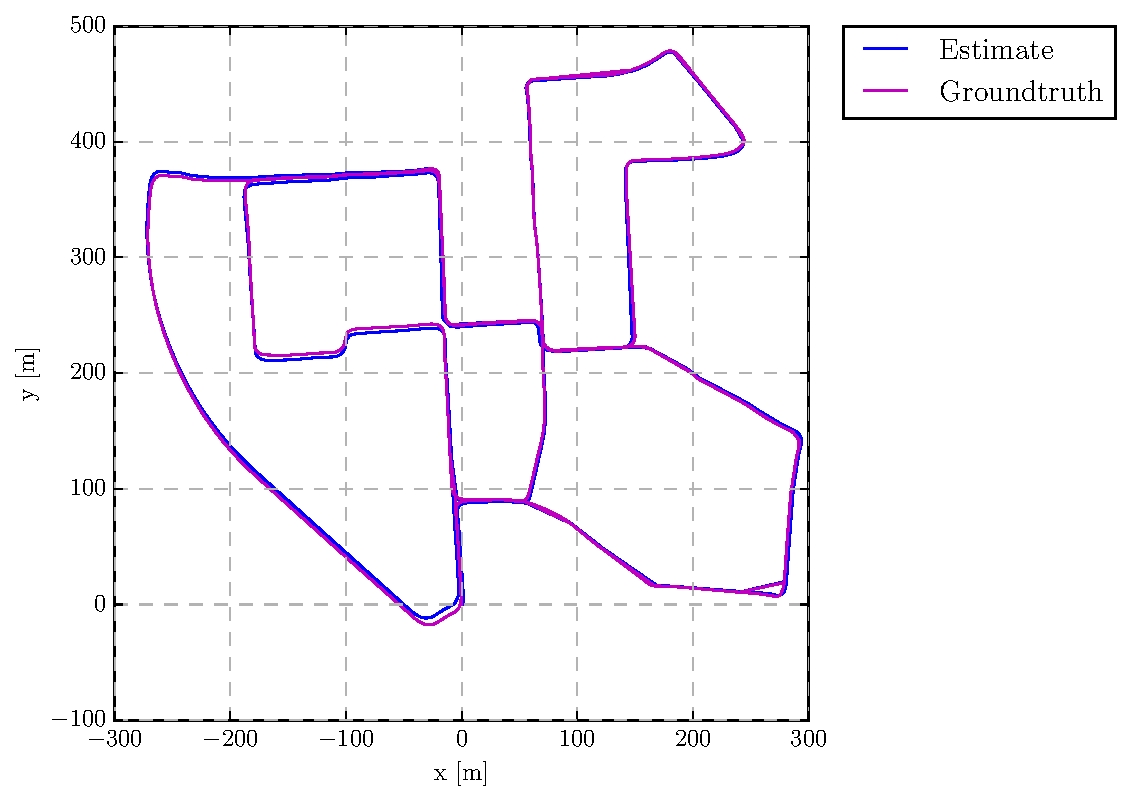
\includegraphics[width=5in]{Chapter4/KITTI/00server/plots/trajectory_side_sim3_-1.pdf}
			%\caption{fig1}
		\end{minipage}
	}
	\caption{Mapping results of Seq.0 and Seq.1, and the map fusion results of KITTI Datasets.}
	\label{fig:kittiresults}
\end{figure}

\begin{figure}
	\centering
	\subfigure[Relative translation error.]{
		\label{sfig:kittireltran}
		\begin{minipage}[t]{0.4\linewidth}
			\centering
			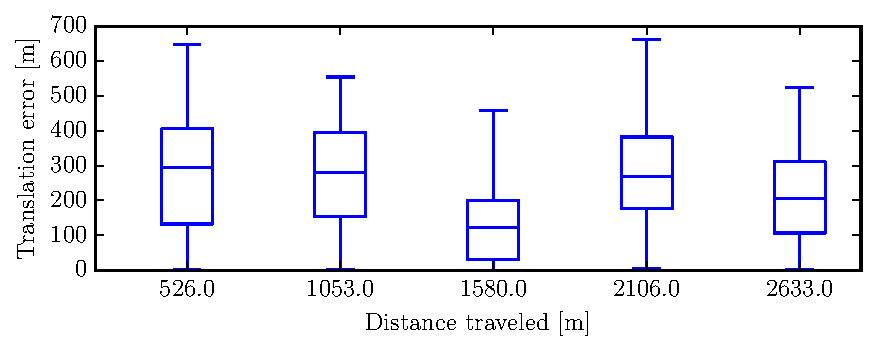
\includegraphics[width=2in]{Chapter4/KITTI/00server/plots/rel_translation_error.pdf}
			%\caption{fig1}
		\end{minipage}
	}
	\subfigure[Relative translation error by percent.]{
		\label{sfig:kittireltranper}
		\begin{minipage}[t]{0.4\linewidth}
			\centering
			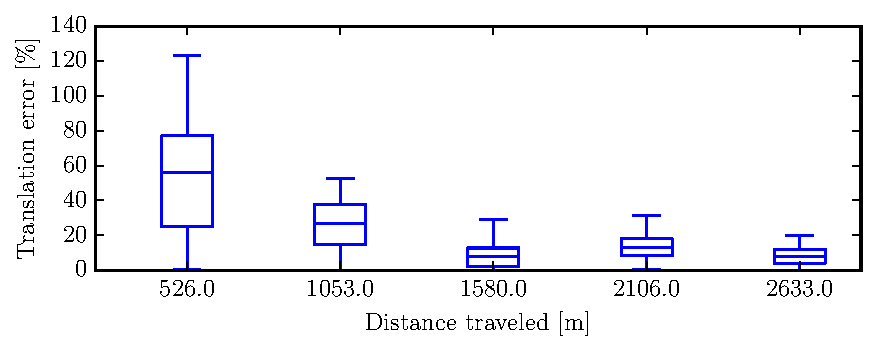
\includegraphics[width=2in]{Chapter4/KITTI/00server/plots/rel_translation_error_perc.pdf}
			%\caption{fig2}
		\end{minipage}
	}
	\vfill
	\subfigure[Relative yaw error.]{
		\label{sfig:kittirelyaw}
		\begin{minipage}[t]{0.4\linewidth}
			\centering
			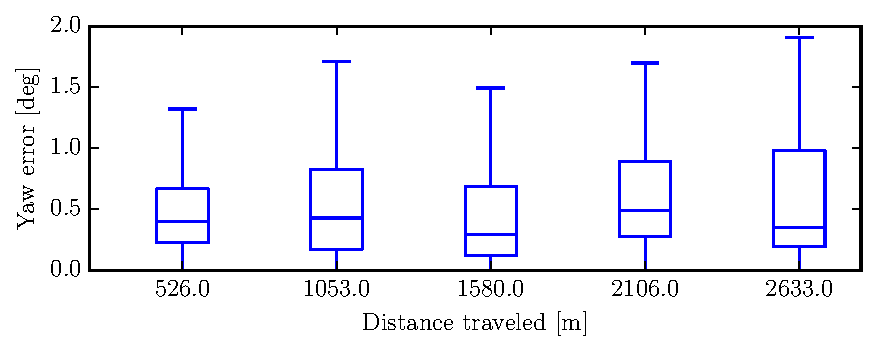
\includegraphics[width=2in]{Chapter4/KITTI/00server/plots/rel_yaw_error.pdf}
			%\caption{fig1}
		\end{minipage}
	}
	\subfigure[Scale error.]{
		\label{sfig:kittiscaleerr}
		\begin{minipage}[t]{0.4\linewidth}
			\centering
			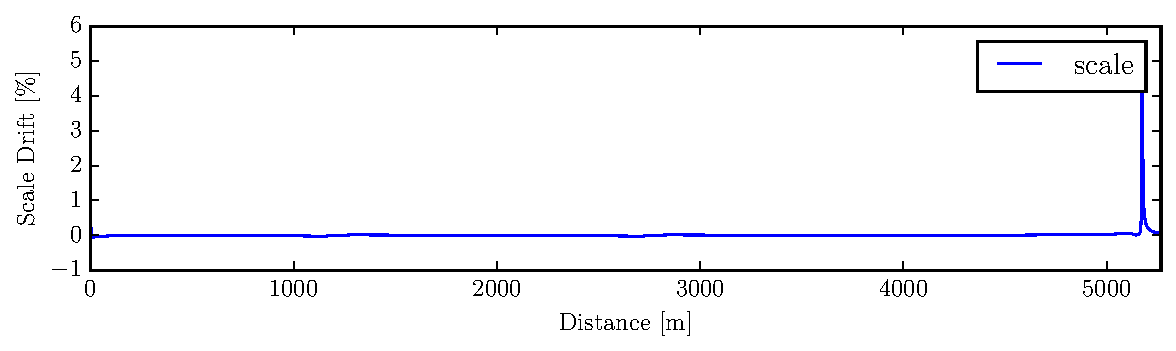
\includegraphics[width=2in]{Chapter4/KITTI/00server/plots/scale_error_sim3_-1.pdf}
			%\caption{fig2}
		\end{minipage}
	}
	\caption{Quantitative evaluation results of fused map of KITTI Datasets.}
	\label{fig:kittiquanresult}
\end{figure}

\begin{table*}
	\centering
	\caption{Quantitative results of map fusion evaluation on KITTI partial sequences.}
	\begin{threeparttable}
	\begin{tabular}{|c|c|c|c|c|}
		\hline
		Distance(m)\tnote{1} & Rel. Trans.(m)\tnote{2}  & Rel. Trans.($\%$)\tnote{3} & Rel. Yaw(deg)\tnote{4} & Scale Err.($\%$)\tnote{5}  \\
		\hline
		526& 283.40 & 53.88 & 0.46& - \\
		\hline
		1053&276.16& 26.23 & 0.51 & - \\
		\hline
		1580&153.74& 9.73 & 0.48 & - \\
		\hline
		2106&284.95& 13.53 & 0.57 & - \\
		\hline
		2633&219.66& 8.34 & 0.54 & - \\
		\hline
		-&-&- & - &  -0.15\\
		\hline
	\end{tabular}
      \begin{tablenotes}
		\footnotesize
		\item[1] Distance in meter traveled before each time of statistics. 
		\item[2] Mean relative translation error in meter.
		\item[3] Mean relative translation error in percent.
		\item[4] Mean relative yaw error in degree.
		\item[5] Median scale error in percent.
	\end{tablenotes}
	\end{threeparttable}
	\label{tbl:kittiquanresult}
\end{table*}

\subsubsection{NTU Datasets}

An obvious drawback of the evaluation on KITTI dataset is the images which are overlapped by two clients are exactly identical because they are extracted from the same sequence. Therefore, the results are expected to be much better than real-world applications in which case it is impossible the images recorded by different clients can be identical.

In order to get more reliable and convincing evaluation results of  CORB-SLAM system, another evaluation on multi ground robots is performed utilizing NTU Datasets. Bag.0 and Bag.1 described in Section \ref{sec:ntuinfo} are selected in this test. These two bags recorded by two UGVs, have different starting and ending location, with limited overlapping, which is much more similar to the case of real-world applications. Clients' mapping results and map fusion results in the server end compared to ground truth trajectories are demonstrated in Figure \ref{fig:ntubag01serverresults}. And ground truth information is provided in Figure \ref{fig:ntubag01gt} for reference. Quantitative results are represented in Figure \ref{fig:ntuquanresult} and Table \ref{tbl:ntuquanresult}. Results are further discussed in Section \ref{sec:disussmultiground}.

\begin{figure}
	\centering
	\subfigure[Ground truth trajectory of Bag.0.]{
		\begin{minipage}[t]{0.4\linewidth}
			\centering
			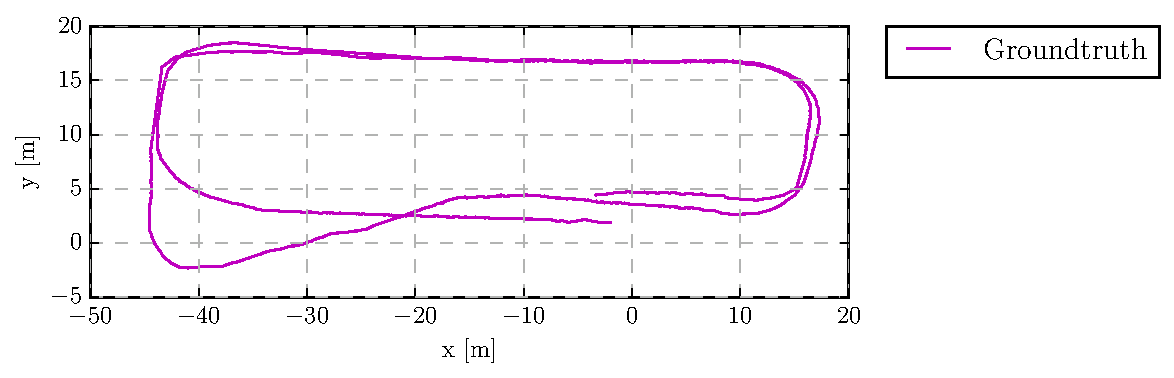
\includegraphics[width=2in]{Chapter4/NTU/0446/trajectory_top_gt_sim3_-1.pdf}
			%\caption{fig1}
		\end{minipage}
	}
	\subfigure[Ground truth trajectory of Bag.1.]{
		\begin{minipage}[t]{0.4\linewidth}
			\centering
			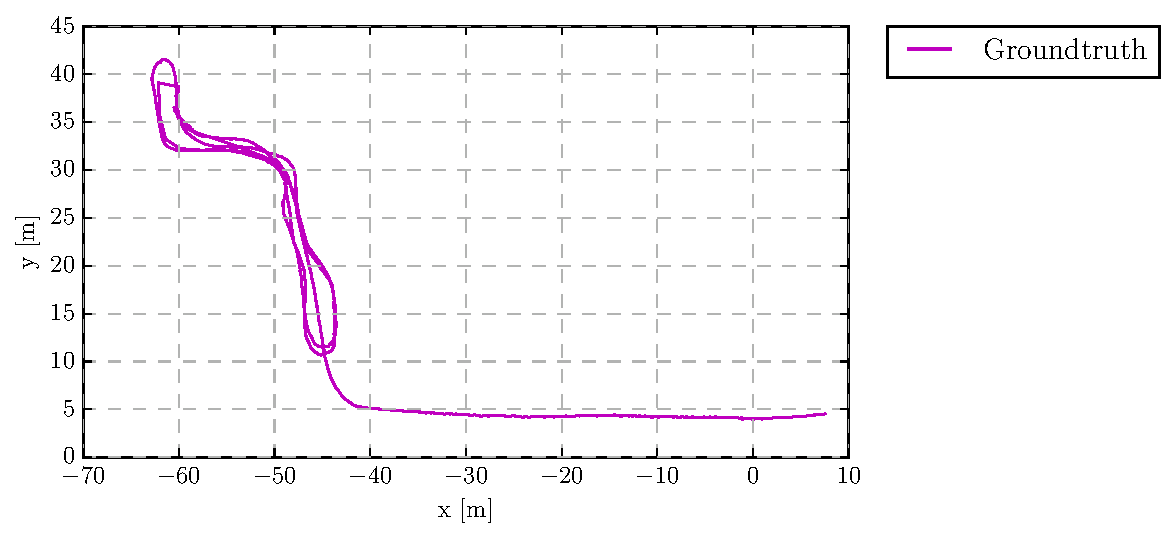
\includegraphics[width=2in]{Chapter4/NTU/0454/trajectory_top_gt_sim3_-1.pdf}
			%\caption{fig2}
		\end{minipage}
	}
	\vfill
	\subfigure[Complete ground truth trajectory of Bag.0 and Bag.1.]{
		\begin{minipage}[t]{\linewidth}
			\centering
			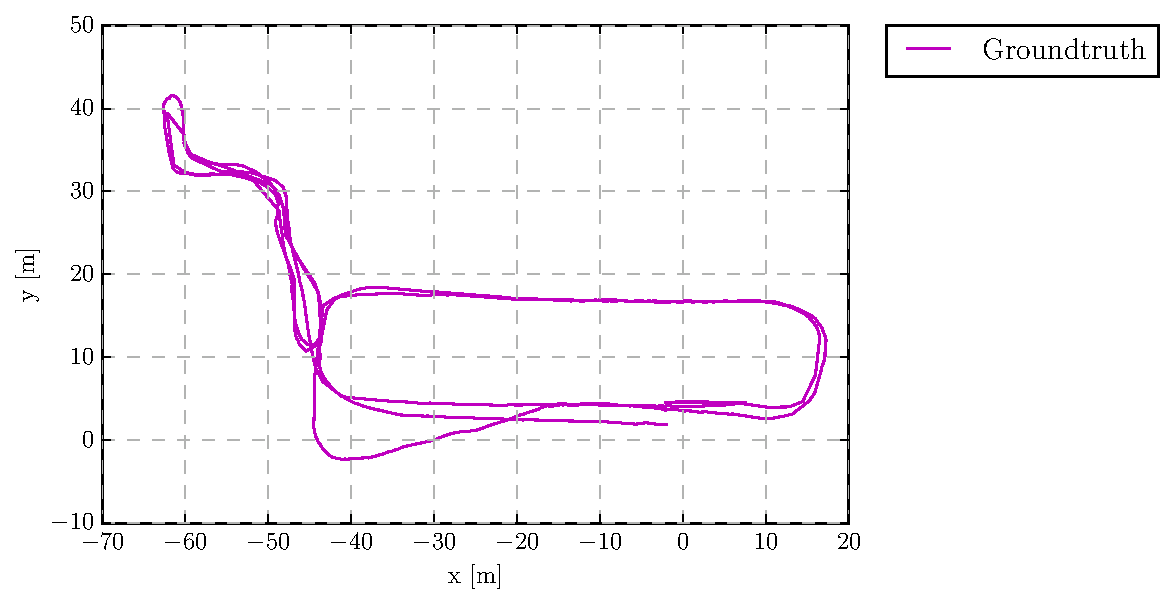
\includegraphics[width=5in]{Chapter4/NTU/server/trajectory_top_gt_sim3_-1.pdf}
			%\caption{fig1}
		\end{minipage}
	}
	\caption{Ground truth trajectory of partial and complete bags of NTU Datasets.}
	\label{fig:ntubag01gt}
\end{figure}

\begin{figure}
	\centering
	\subfigure[Mapping result of Bag.0 compared with ground truth.]{
		\begin{minipage}[t]{0.4\linewidth}
			\centering
			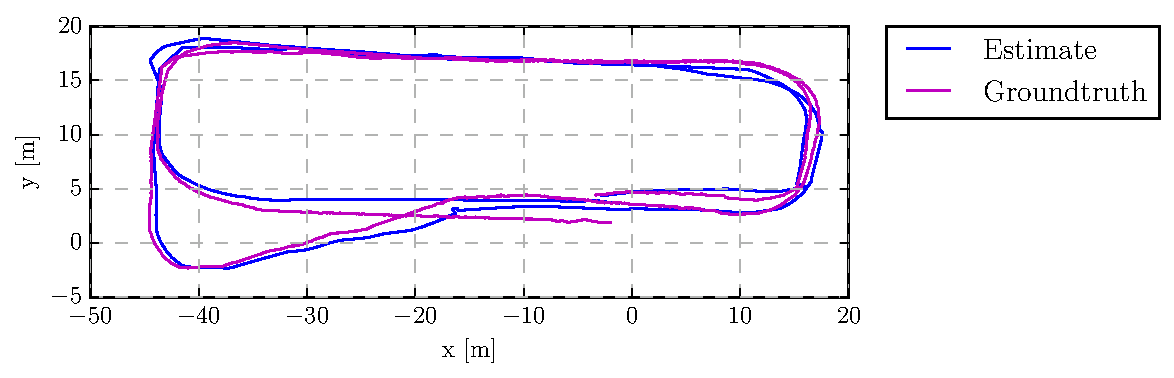
\includegraphics[width=2in]{Chapter4/NTU/0446/trajectory_top_sim3_-1.pdf}
			%\caption{fig1}
		\end{minipage}
	}
	\subfigure[Mapping result of Bag.1 compared with ground truth.]{
		\begin{minipage}[t]{0.4\linewidth}
			\centering
			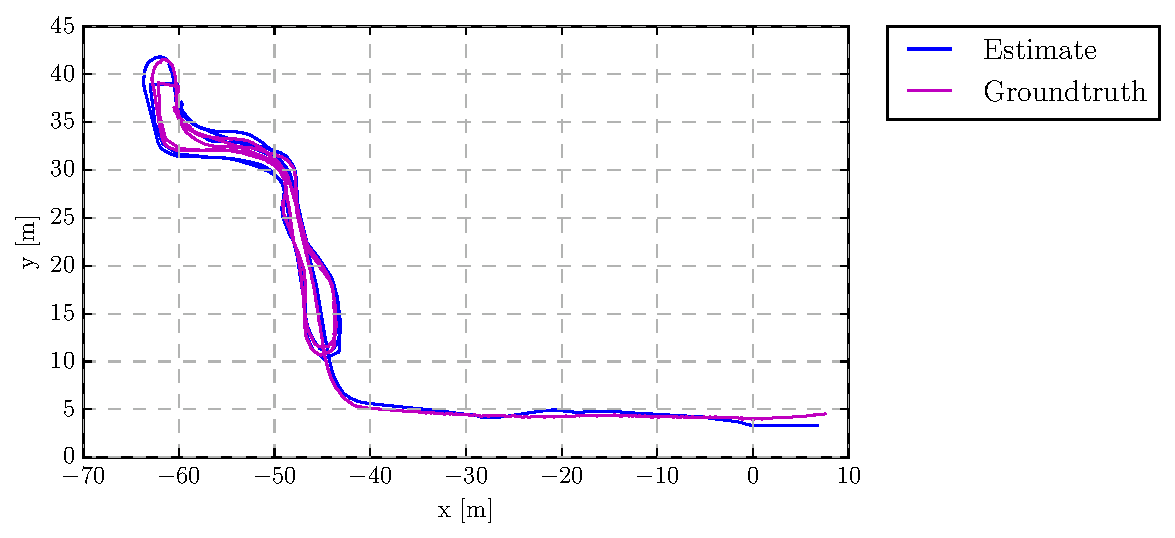
\includegraphics[width=2in]{Chapter4/NTU/0454/trajectory_top_sim3_-1.pdf}
			%\caption{fig2}
		\end{minipage}
	}
	\vfill
	\subfigure[Map Fusion results in server end of Bag.0 and Bag.1.]{
		\begin{minipage}[t]{\linewidth}
			\centering
			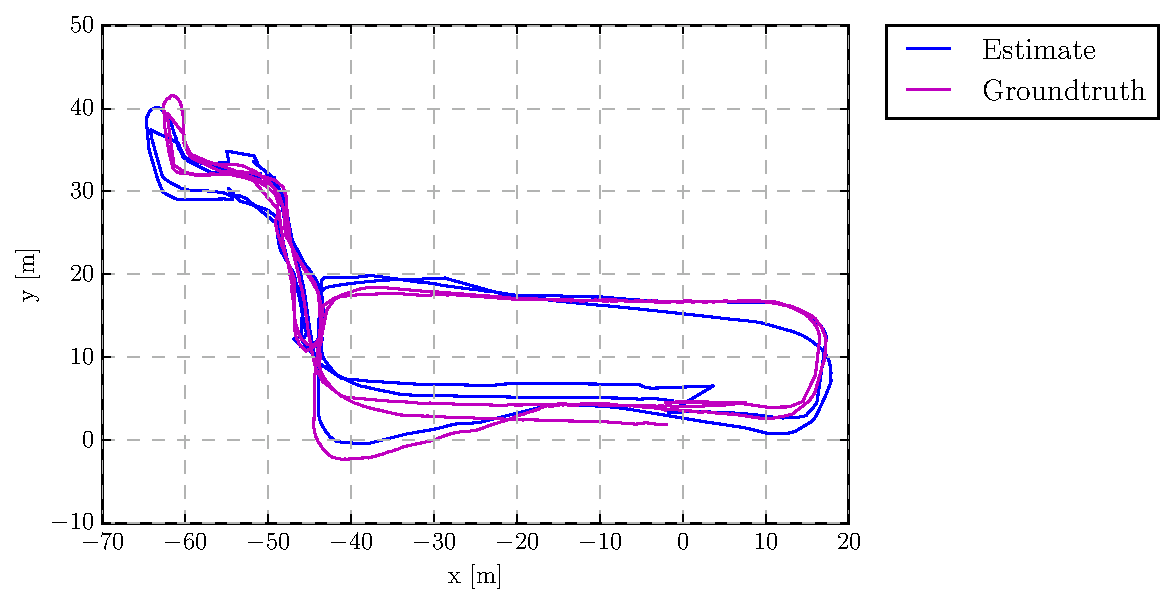
\includegraphics[width=5in]{Chapter4/NTU/server/trajectory_top_sim3_-1.pdf}
			%\caption{fig1}
		\end{minipage}
	}
	\caption{Mapping results of Bag.0 and Bag.1 and the map fusion result of server.}
	\label{fig:ntubag01serverresults}
\end{figure}

\begin{figure}
	\centering
	\subfigure[Relative translation error.]{
		\begin{minipage}[t]{0.4\linewidth}
			\centering
			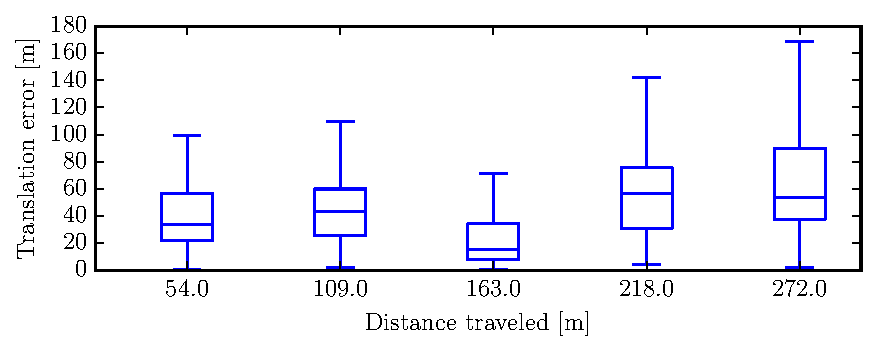
\includegraphics[width=2in]{Chapter4/NTU/server/rel_translation_error.pdf}
			%\caption{fig1}
		\end{minipage}
	}
	\subfigure[Relative translation error by percent.]{
		\begin{minipage}[t]{0.4\linewidth}
			\centering
			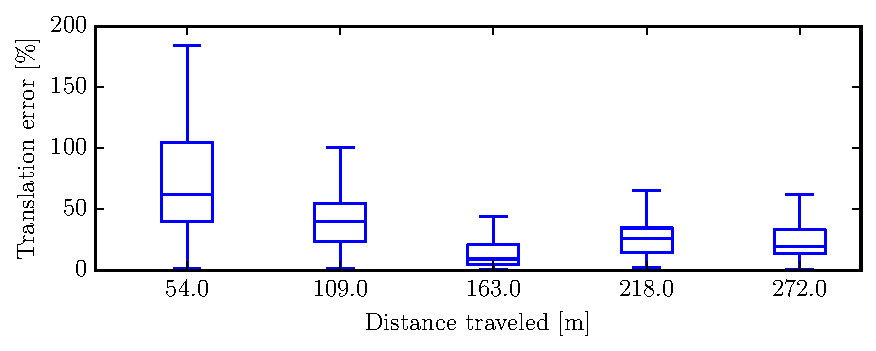
\includegraphics[width=2in]{Chapter4/NTU/server/rel_translation_error_perc.pdf}
			%\caption{fig2}
		\end{minipage}
	}
	\vfill
	\subfigure[Relative yaw error.]{
		\begin{minipage}[t]{0.4\linewidth}
			\centering
			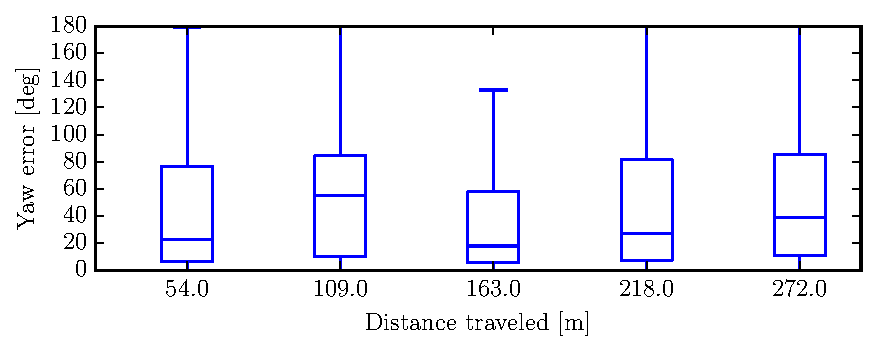
\includegraphics[width=2in]{Chapter4/NTU/server/rel_yaw_error.pdf}
			%\caption{fig1}
		\end{minipage}
	}
	\subfigure[Scale error.]{
		\begin{minipage}[t]{0.4\linewidth}
			\centering
			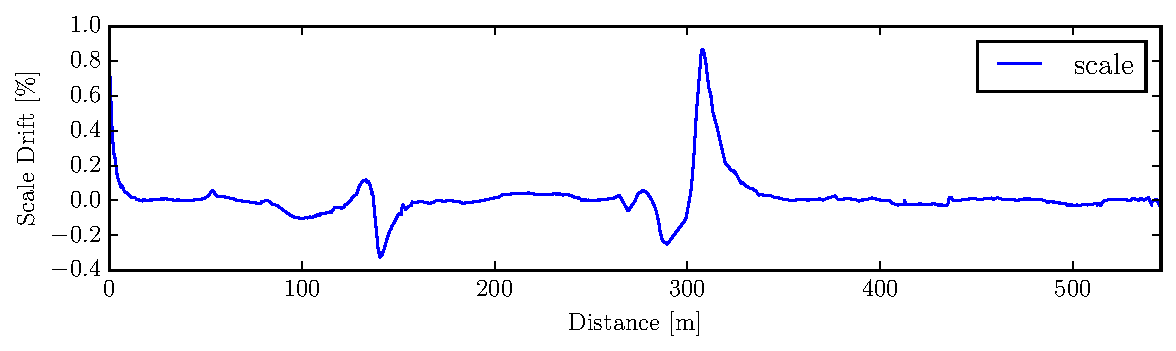
\includegraphics[width=2in]{Chapter4/NTU/server/scale_error_sim3_-1.pdf}
			%\caption{fig2}
		\end{minipage}
	}
	\caption{Quantitative evaluation results of fused map of NTU Datasets.}
	\label{fig:ntuquanresult}
\end{figure}

\begin{table*}
	\centering
	\caption{Quantitative results of evaluation on NTU Datasets.}
	\begin{threeparttable}
		\begin{tabular}{|c|c|c|c|c|}
			\hline
			Distance(m)\tnote{1} & Rel. Trans.(m)\tnote{2}  & Rel. Trans.($\%$)\tnote{3} & Rel. Yaw(deg)\tnote{4} & Scale Err.($\%$)\tnote{5}  \\
			\hline
			54& 39.38 & 72.93 & 44.39& - \\
			\hline
			109&44.88& 41.18 & 57.01 & - \\
			\hline
			163&26.09& 16.00 & 32.12 & - \\
			\hline
			218&54.99& 25.23 & 46.11 & - \\
			\hline
			272&64.66& 23.77 & 54.65 & - \\
			\hline
			-&-&- & - &  0.10\\
			\hline
		\end{tabular}
		\begin{tablenotes}
			\footnotesize
			\item[1] Distance in meter traveled before each time of statistics. 
			\item[2] Mean relative translation error in meter.
			\item[3] Mean relative translation error in percent.
			\item[4] Mean relative yaw error in degree.
			\item[5] Median scale error in percent.
		\end{tablenotes}
	\end{threeparttable}
	\label{tbl:ntuquanresult}
\end{table*}

\subsection{Evaluation on multi hybrid robots}
The evaluation of 

\section{Evaluation under different illumination}
\subsubsection{Oxford RobotCar Datasets}
CORB-SLAM system integrated with illumination variance is firstly evaluated on the selected sequences of Oxford RobotCar Datasets, and then the mapping results are compared with the ground truth trajectories, with quantitative evaluation results calculated.

Two partial sequences are selected according the following principles: 
\begin{enumerate}[1.]
	\item Exclude the overexposed photo, which will cause tracking lost in ORBSLAM system.
	Because the dataset was collected in real-world outdoor street environment, there are some frames with overexposure e.g. Figure \ref{fig:robotcaroverexposed}, which cannot be process by vSLAM. Therefore, in this work, this dataset is intercepted into two sub sequences excluding overexposed images.

	\begin{figure}[H]
		\centering
		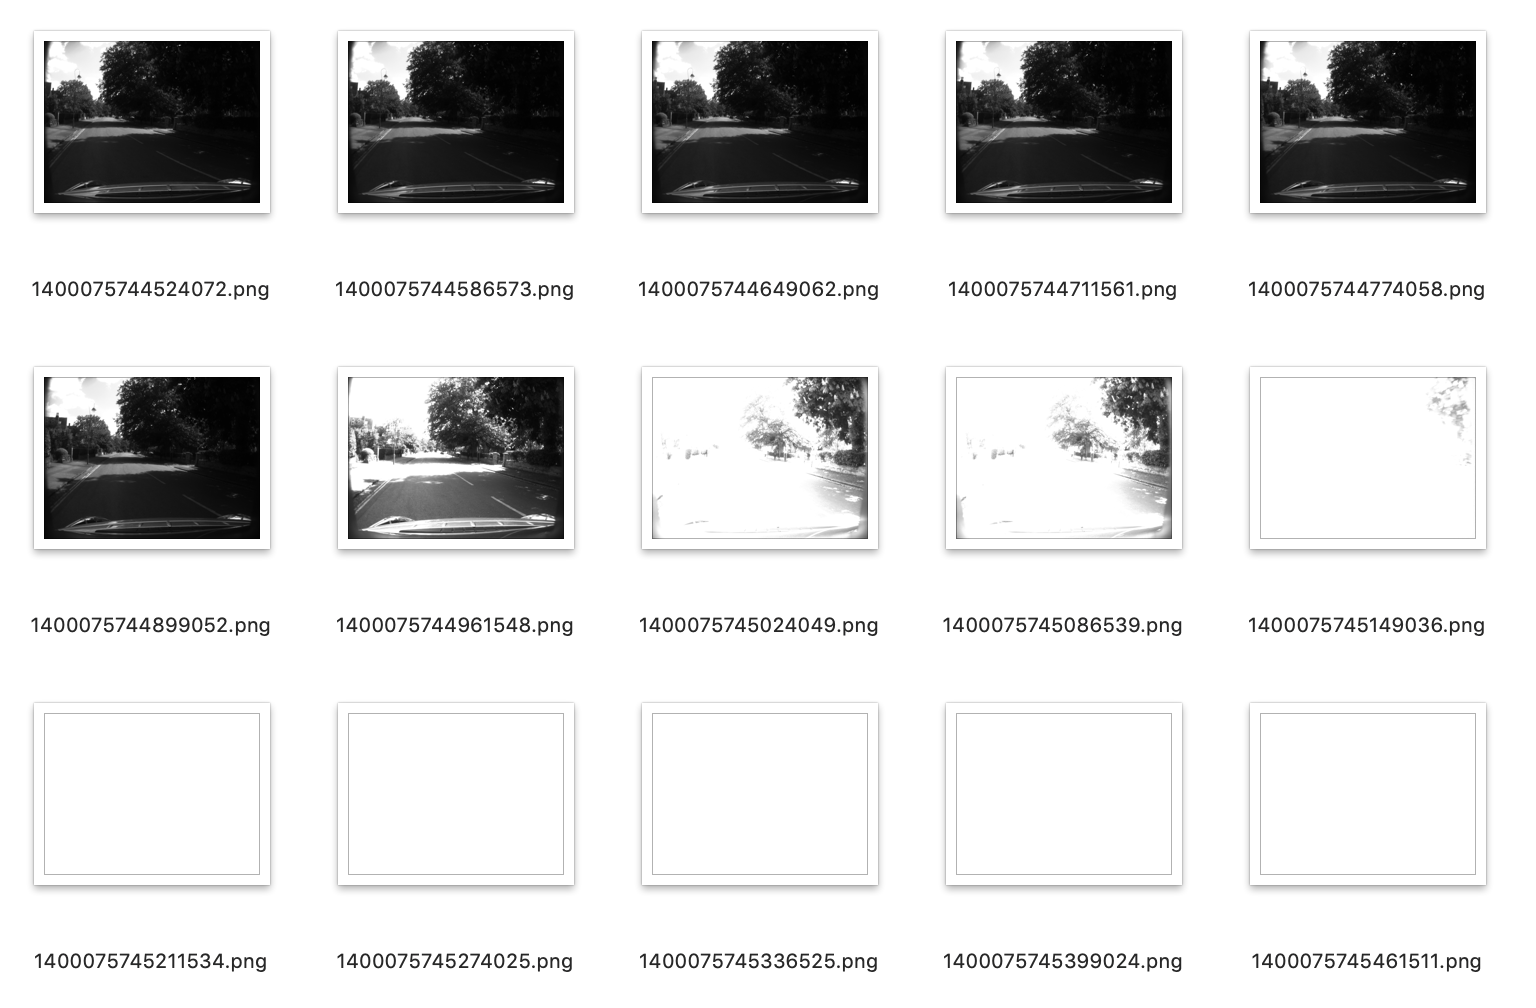
\includegraphics[width=5in]{Chapter4/robotcaroverexposed.eps}
		\caption{Image sequence with overexposed frames in RobotCar dataset.}
		\label{fig:robotcaroverexposed} 
	\end{figure}

	\item Avoid partial sequences where traffic congestion occurred. Because RobotCar Datasets are recorded in different hours during daytime, there are congestion starting at approximately 15:00, as shown in   
	
\begin{figure}[H]
	\centering
	
\includegraphics[width=5in]{thereisafigure.eps}
	\caption{Images when traffic congestion occurred in RobotCar datasets.}
	\label{fig:robotcarcongestion} 
\end{figure}

	\item Select partial sequence containing images with overlapping under different illumination conditions and in different season, as shown in Figure \ref{fig:robotcarcomparisonseason}. 
\end{enumerate}

According to the above selection principles, the two sub sequences selected are listed in Table \ref{tbl:robotcarpartial}. The ground truth GPS/INS trajectories of two sub sequences and the combined overall trajectories are shown in Figure \ref{fig:robotcarseq01servergt}. The estimate trajectories and the fused map of two partial sequences are shown in Figure \ref{fig:robotcarseq01serverresults}. Results of Oxford RobotCar Datasets are further discussed in Section \ref{sec:discusslifelong}.

\begin{table*}
	\centering
	\caption{Partial datasets selected in RobotCar dataset.}
	\begin{tabular}{|c|c|c|c|c|}
		\hline
		Seq. No. & Data(M/D/Y) & Time & Weather & Timestamps  \\
		\hline
		0&07/14/2014&14:49&\tabincell{c}{summer\\overcast}& \tabincell{c}{1405349847738682 to\\1405350059147905}\\
		\hline
		1&02/24/2014&12:32&\tabincell{c}{winter\\overcast}& \tabincell{c}{1417794166325288 to\\1417794407042717}\\
		\hline
	\end{tabular}
	\label{tbl:robotcarpartial}
\end{table*}

\begin{figure}
	\centering
	\subfigure[Ground truth trajectory of Seq.0.]{
		\begin{minipage}[t]{0.4\linewidth}
			\centering
			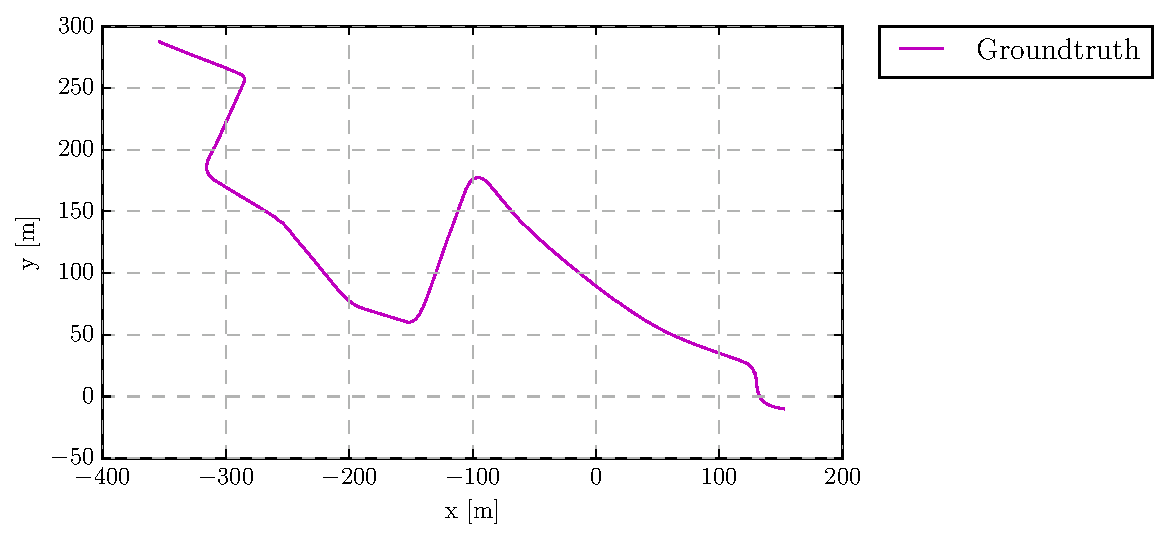
\includegraphics[width=2in]{Chapter3/0714gt.pdf}
			%\caption{fig1}
		\end{minipage}
	}
	\subfigure[Ground truth trajectory of Seq.0.]{
		\begin{minipage}[t]{0.4\linewidth}
			\centering
			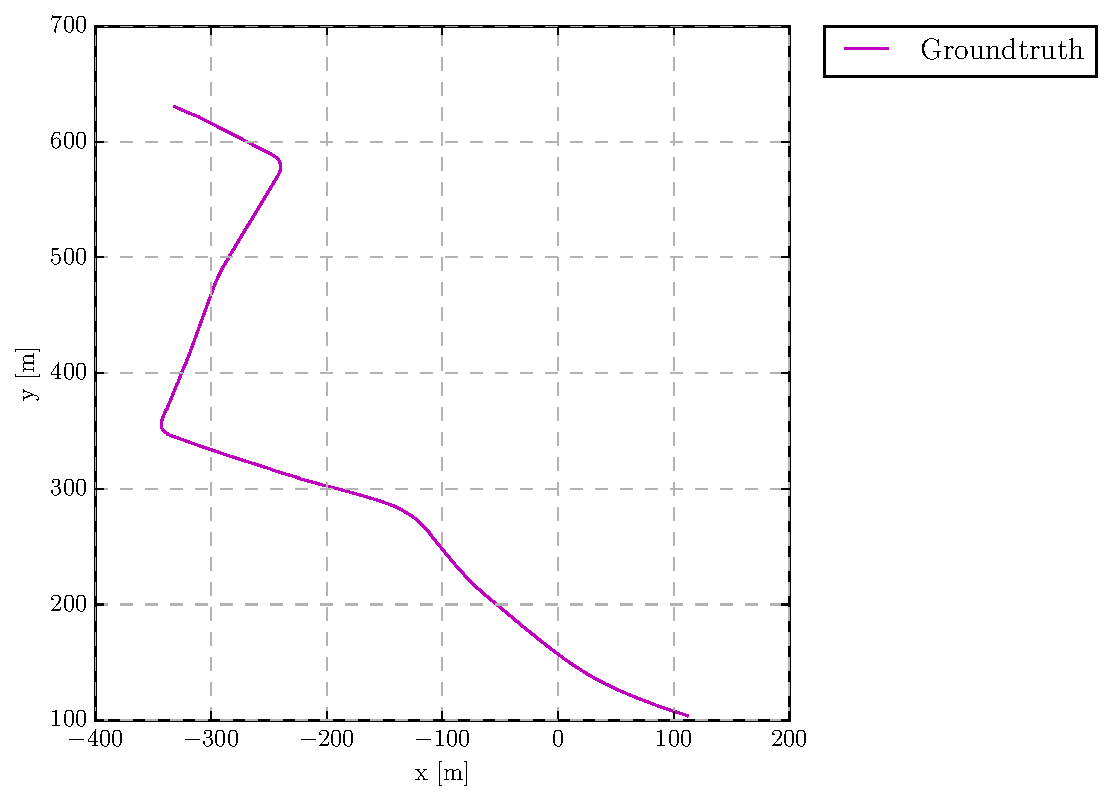
\includegraphics[width=2in]{Chapter3/0224gt.pdf}
			%\caption{fig2}
		\end{minipage}
	}
	\vfill
	\subfigure[Overall ground truth trajectory of Seq.0 and Seq.1.]{
		\begin{minipage}[t]{\linewidth}
			\centering
			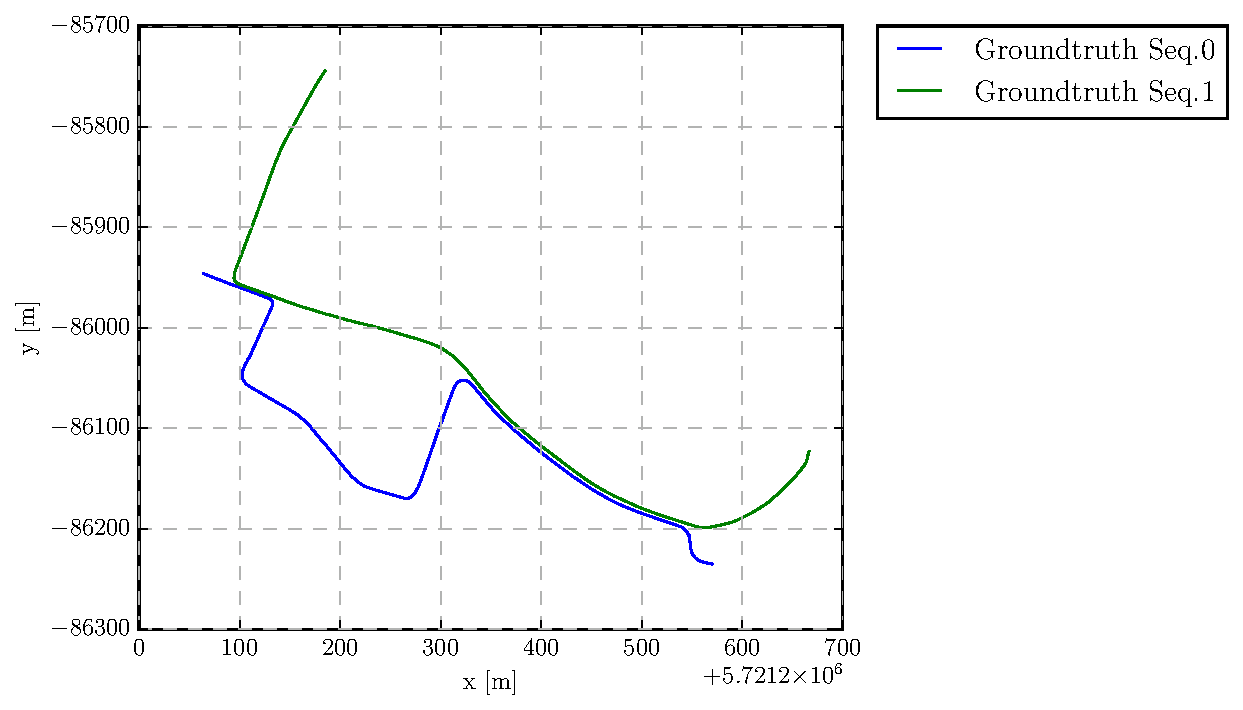
\includegraphics[width=5in]{Chapter3/overall_gt_top_.pdf}
			%\caption{fig1}
		\end{minipage}
	}
	\caption{Ground truth individual and overall trajectories of Seq.0 and Seq.1 in Oxford RobotCar Datasets.}
	\label{fig:robotcarseq01servergt}
\end{figure}

\begin{figure}
	\centering
	\subfigure[Mapping result of Seq.0.]{
		\begin{minipage}[t]{0.4\linewidth}
			\centering
			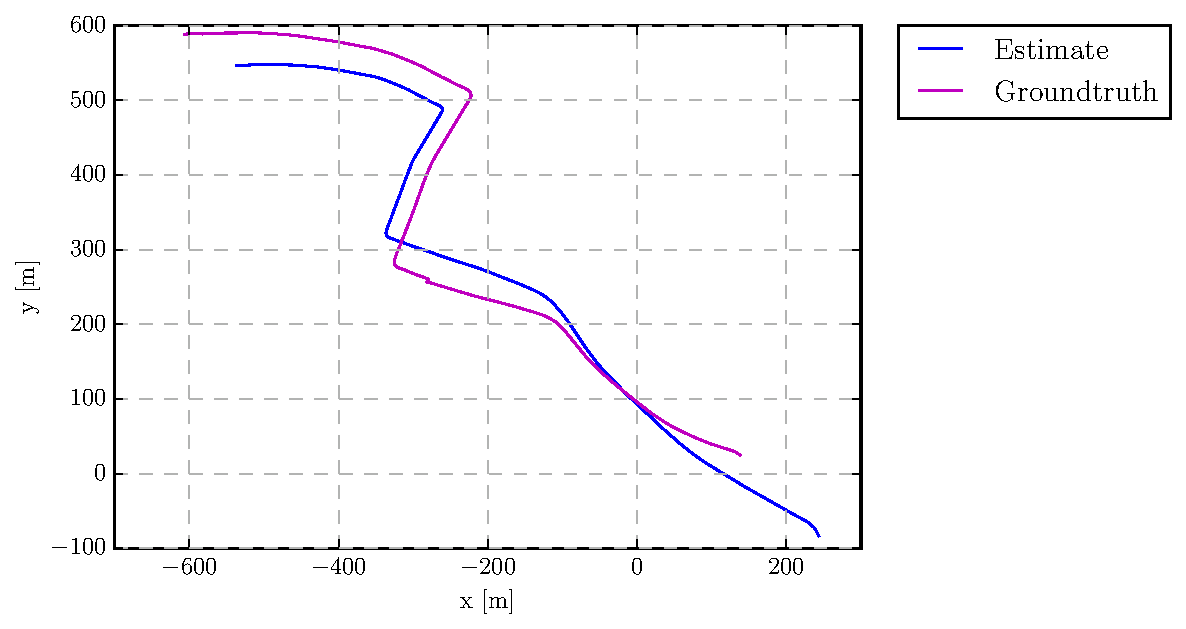
\includegraphics[width=2in]{Chapter4/robotcar/0714/gps/plots/trajectory_top_sim3_-1.pdf}
			%\caption{fig1}
		\end{minipage}
	}
	\subfigure[Mapping result of Seq.1.]{
		\begin{minipage}[t]{0.4\linewidth}
			\centering
			\includegraphics[width=2in]{Chapter4/robotcar/0224/gps/plots/trajectory_top_sim3_-1.pdf}
			%\caption{fig2}
		\end{minipage}
	}
	\vfill
	\subfigure[Map Fusion results in server end of Seq.0 and Seq.1.]{
		\begin{minipage}[t]{\linewidth}
			\centering
			\includegraphics[width=5in]{Chapter4/robotcar/plots/trajectory_top_sim3_-1.pdf}
			%\caption{fig1}
		\end{minipage}
	}
	\caption{Mapping results of Seq.0 and Seq.1 and the map fusion result of server in Oxford RobotCar Datasets.}
	\label{fig:robotcarseq01serverresults}
\end{figure}

\begin{figure}[H]
	\centering
	\includegraphics[width=5in]{Chapter4/robotcar/plots/trajectory_top_est_sim3_-1.pdf}
	\caption{Map fusion results of Seq.0 and Seq.1 without ground truth in Oxford RobotCar Datasets.}
	\label{fig:robotcarmfresult} 
\end{figure}


%=== END OF CHAPTER FOUR ===
\newpage

%=== CHAPTER FIVE (5) ===
%=== Discussion ===

\chapter{Discussion}

\section{Results of multi ground robots cluster}
\label{sec:disussmultiground}

Seen graphically according to Figure \ref{fig:kittiresults}, the mapping results of CORB-SLAM clients is able to match the ground truth trajectory fairly well enough. And seeing the numeric analysis in Table \ref{tbl:kittiquanresult}, the completed map fused by the server has $8.34\%$ mean relative translation error and $0.54^\circ$ mean relative yaw error with all distance traveled.

Comparing the fused map with the mapping results on the original unseparated sequence, according to the differences between Table \ref{tbl:kittiquanresult} and \ref{tbl:kitticlientquanresult}, map fusion in CORB-SLAM server slight reduces the accuracy on relative yaw and scaling. However from the table, the relative translation accuracy is numerically increased, of which a critical reason is the distance traveled by each client is inevitable shortened because the sequence is divided into two parts, which means translation errors on each client are accumulated during shorter distances. Therefore, it is not concluded so far that map fusion module in server can increase accuracy of relative translation.

Evaluation on KITTI Dataset is an ideal circumstance, with all overlapped images identical. To evaluate under a more general real-world circumstance to get more universal and convincing results, another evaluation is performed utilizing NTU Dataset. 

According to the comparison of quantitative map fusion result ( in Figure \ref{fig:ntuquanresult} and Table \ref{tbl:ntuquanresult} ) and mapping results of single bags ( in Figure \ref{fig:ntubag0quanresult}, \ref{fig:ntubag1quanresult} and Table \ref{tbl:ntubag0quanresult}, \ref{tbl:ntubag1quanresult} ), compared to 6.32$\%$ relative translation error of client of Bag.0, and 30.70$\%$ of Bag.1, the global fused map in server has an error of 23.77$\%$, which can be considered as an acceptable result, considering Bag.1 has a complicated trajectory consisting both parts of indoor and outdoor environment causing client map has a relatively higher translation error.

%\section{Results of multi hybrid robots cluster}
%\label{sec:disussmultihybrid}

\section{Failure Reasons and Drawbacks of Illumination Variance Method}
\label{sec:discusslifelong}

According to the ground truth information of the selected partial sequences of Oxford RobotCar Datasets, the correct fused estimate trajectories of clients should be coincident with very little offset seen as Figure \ref{fig:robotcarseq01servergt}. However as shown in Figure \ref{fig:robotcarmfresult}, integrating CORB-SLAM system with illumination variance failed to enhance the ability to deal with illumination and season changes in Oxford RobotCar Datasets. 

As seen in Figure \ref{fig:robotcarmfresult}, illumination variance method introduce many incorrect matches of keypoints while it is expected to allow ORB matcher to find more correct keypoint pairs that hard to match in raw images due to illumination changes. 

By analyzing the basic formula to compute illumination variance, Equation \ref{eq:iifinal} which is repeated below as Equation \ref{eq:discussiifinal} for reference, and the result images in Figure \ref{fig:discussrobotcarill}, the following reasons and drawbacks of illumination variance method can be concluded to explain the failure of it to help CORB-SLAM deal with images under different illumination conditions and seasons: 

\begin{equation}
I=\log(R)-\alpha\log(G)-(1-\alpha)\log(B)
\label{eq:discussiifinal}
\end{equation}

\begin{enumerate}[1.]
	\item Loss of resolution. According to the computation shown in Equation \ref{eq:discussiifinal}, there are two steps in this method to calculate the value of illumination variance: for each pixel, 
		\begin{inparaenum}[1)]
			\item logarithm of r,g, b channel values,
			\item take their weighted difference as the result illumination variance value.
		\end{inparaenum}
	Both steps cause serious loss of resolution, with the result image very blurry as seen in Figure \ref{fig:discussrobotcarill}. 
	
	\item Requirement of high brightness and contrast of input color images. In Figure \ref{fig:discussrobotcarill}, compared to Figure \ref{sfig:robotcarjulyill}, Figure \ref{sfig:robotcarjulyill} has a higher resolution. This is because with the loss of resolution during the illumination variance computation, images with higher brightness and contrast can remain more details in the result images. But the background of application of this method is in long-term localization and mapping system, running under significant lighting and season conditions, which means it is an unreasonable request to demand the input images always bright and sharp.
	
%	\item Because of loss of resolution, obviously the position information of keypoints in illumination variance images are not accurate enough to estimate trajectories within acceptable errors. To solve this problem, the initial idea in this work is when close loops are detected in illumination variance images, the visual odometer module 
\end{enumerate}


\begin{figure}
	\centering
	\subfigure[Corresponding illumination variance image of Figure \ref{sfig:robotcarjulyraw}.]{
		\begin{minipage}[t]{\linewidth}
			\label{sfig:robotcarjulyill}
			\centering
			\includegraphics[width=4in]{Chapter4/robotcar/ill_inv1.eps}
			%\caption{fig1}
		\end{minipage}
	}
\vfill
	\subfigure[Corresponding illumination variance image of Figure \ref{sfig:robotcarfebraw}.]{
		\begin{minipage}[t]{\linewidth}
			\label{sfig:robotcarfebill}
			\centering
			\includegraphics[width=4in]{Chapter4/robotcar/ill_inv2.eps}
			%\caption{fig2}
		\end{minipage}
	}
	\caption{Generated illumination variance images of example raw images in Oxford RobotCar Datasets.}
	\label{fig:discussrobotcarill}
\end{figure}

\begin{figure}[H]
	\centering
	\subfigure[Corresponding matched keypoint pairs of raw images Figure \ref{sfig:robotcarjulyraw} and \ref{sfig:robotcarfebraw}.]{
		\begin{minipage}[t]{\linewidth}
			\centering
			\includegraphics[width=5in]{Chapter4/robotcar/rawmatches.eps}
			\label{sfig:discussrobotcarrawmatch}
		\end{minipage}
	}
	\vfill
	\subfigure[Corresponding matched keypoint pairs of illumination variance images Figure \ref{sfig:robotcarjulyill} and \ref{sfig:robotcarfebill}.]{
		\begin{minipage}[t]{\linewidth}
			\centering
			\includegraphics[width=5in]{Chapter4/robotcar/matches.eps}

			\label{sfig:discussrobotcarillmatch}
		\end{minipage}
	}
\caption{ORB Keypoint matching results of raw and illumination variance images in Oxford RobotCar Datasets.}
\label{fig:robotcarmatches}
\end{figure}

However, in both the original work \cite{maddern2014illumination} and the related implement in \cite{arroyo2014bidirectional,arroyo2014fast,arroyo2015towards,arroyo2016openable}, the application of this method only focus on localization, which means the main function is designed to detect loop closures in images taken in different illumination and seasons, but not suitable for mapping. In all above papers, evaluation results are given only by localization results.

A critical difference of localization and mapping tasks is high resolution images are not necessary in localization, while in mapping task they are. Cited by \cite{arroyo2014bidirectional}, \cite{milford2012visual}  explains that performing localization using a sequence of images rather than single image removes the requirement that the image matching scheme be able to reliably calculate a single global image match. However, without the functionality of calculating matches between single images, sequence-based image matching algorithms have significant drawbacks that cannot calculate the transformation between images.

And in the case of CORB-SLAM, the image matching algorithm combing ORB keypoint and Bag of Words, is able to calculate matching and transformation between individual images, but fit not well with illumination variance method.

%=== END OF CHAPTER FIVE ===
\newpage

%=== CHAPTER SIX (6) ===
%=== Conclusion and Recommendations ===

\chapter{Conclusion and Recommendations}

\section{One}

\section{Two}

\section{Three}


%=== END OF CHAPTER SIX ===
\newpage

%==== ENDING PART ===

\bibliographystyle{unsrt}
\bibliography{Ref/refs.bib}

%=== APPENDIX ===
%=== APPENDIX ===

\chapter*{Appendix: Example Code}
\addcontentsline{toc}{chapter}{Appendix: Example Code}
\label{sec:appendixa}

\subsubsection{Map Fuse To Global Map}

\definecolor{mGreen}{rgb}{0,0.6,0}
\definecolor{mGray}{rgb}{0.5,0.5,0.5}
\definecolor{mPurple}{rgb}{0.58,0,0.82}
\definecolor{backgroundColour}{rgb}{0.95,0.95,0.92}

\lstdefinestyle{CStyle}{
	backgroundcolor=\color{backgroundColour},   
	commentstyle=\color{mGreen},
	keywordstyle=\color{magenta},
	numberstyle=\tiny\color{mGray},
	stringstyle=\color{mPurple},
	basicstyle=\footnotesize,
	breakatwhitespace=false,         
	breaklines=true,                 
	captionpos=b,                    
	keepspaces=true,                 
	numbers=left,                    
	numbersep=5pt,                  
	showspaces=false,                
	showstringspaces=false,
	showtabs=false,                  
	tabsize=2,
	language=C
}


\begin{lstlisting}[style=CStyle]
bool MapFusion::mapFuseToGlobalMap(ServerMap *sMap) {
	// if global map is null, this submap is inserted into the global map and does not do transform
	{
		std::unique_lock<mutex> lock( nullGlobalMapMutex );
		if( ifNullGlobalMap ) {
		
			cv::Mat Tnorm = cv::Mat::eye(4,4, CV_32F);
			std::unique_lock<mutex> lock(mSubMapUpdatedMutex);
			insertServerMapToGlobleMap(sMap, Tnorm);
			ifSubToGlobalMap[(*sMap).pCacher->pClientId] = true;
			subMapTransM[(*sMap).pCacher->pClientId] = Tnorm;
			pubToClient->transMs[ (*sMap).pCacher->pClientId ] = Tnorm;
			sMap->clear();
			ifNullGlobalMap = false;
		
			cout <<"Global Map is not null!\n";
			return true;
		}
	}
	
	bool flag = false;
	std::vector<KeyFrame*> allKeyFramesInMapy = sMap->pMap->GetAllKeyFrames();
	
	bool bOK = false;
	std::vector<KeyFrame *> candidateKFs;
	KeyFrame * currentKF;
	
	for( int mit = 0; mit < (int)allKeyFramesInMapy.size(); mit++ ) {
	
		KeyFrame * tKF = allKeyFramesInMapy[mit];
		
		cv::Mat oldTwc = tKF->GetPoseInverse();
		cv::Mat oldTcw = tKF->GetPose();
		cv::Mat newTcw = cv::Mat::eye(4,4, newTcw.type());
		
		candidateKFs.clear();
		currentKF = tKF;
		
		bOK = detectKeyFrameInServerMap( globalMap, tKF, newTcw, candidateKFs);
		
		if( bOK ) {
		
			mpGBA->setCurentKeyFrame( currentKF );
			
			mpGBA->setCandidates( candidateKFs );
			
			if( mpGBA->ComputeSim3() ) {
			
				ROS_INFO("Detect In serverMap[%d], from keyframe id[%d]", 
				(int)sMap->pCacher->pClientId, (int)tKF->mnId);
				// if this keyframe is deteted in the serverMapx
			
				cv::Mat To2n = oldTwc * newTcw;
				cv::Mat Tnorm = cv::Mat::eye(4,4, newTcw.type());
			
				flag = true;
			
				subMapTransM[ (*sMap).pCacher->pClientId ] = To2n;
				pubToClient->transMs[ (*sMap).pCacher->pClientId ] = To2n;
				ifSubToGlobalMap[ (*sMap).pCacher->pClientId ] = true;
				insertServerMapToGlobleMap( sMap, To2n );
				sMap->clear();
			}
			
			mpGBA->CorrectLoop();
			
			time_t end_t = clock();
			
			cout << "mapfuse " << globalMap->pMap->KeyFramesInMap() << " " << allKeyFramesInMapy.size() << " " << (double)( end_t - start_t )/(double)CLOCKS_PER_SEC << endl;
			
			break;
			
			}
			
		}
	
	}
	
	if( flag ){
	resentGlobalMapToClient();
	}
	return flag;
}
\end{lstlisting}

\subsubsection{Illumination Variance Conversion}

\begin{lstlisting}[style=CStyle]
Mat illumination_conversion(Mat image){
	vector<Mat> channels(3);
	split(image, channels);
	
	Mat imageB,imageG,imageR;
	Mat imageI = Mat(Size(image.cols,image.rows),CV_32FC1);
	Mat imageI8U = Mat(Size(image.cols,image.rows),CV_8UC1);
	
	channels[0].convertTo(imageB, CV_32FC1, 1.0/255.0, 0);
	channels[1].convertTo(imageG, CV_32FC1, 1.0/255.0, 0);
	channels[2].convertTo(imageR, CV_32FC1, 1.0/255.0, 0);
	
	float valueG, valueB, valueR;
	for (int i = 0; i < imageI.rows; i++){
	for (int j = 0; j < imageI.cols; j++){
	
			if (imageG.at<float>(i,j) != 0)
				valueG=log(imageG.at<float>(i,j));
			else
				valueG=0;
			
			if (imageB.at<float>(i,j) != 0)
				valueB=alpha*log(imageB.at<float>(i,j));
			else
				valueB=0;
			
			if (imageR.at<float>(i,j) != 0)
				valueR=(1-alpha)*log(imageR.at<float>(i,j));
			else
				valueR=0;
			
			imageI.at<float>(i,j) = 0.5 + valueG - valueB - valueR;
			
			if (imageI.at<float>(i,j)<0) imageI.at<float>(i,j) = 1;
			
		}
	
	}
	
	imageI.convertTo(imageI8U, CV_8UC1, 255.0, 0);
	
	return imageI8U;
}
\end{lstlisting}

%\chapter*{Appendix B: Detailed Table of Quantitative Trajectory Evaluation Results}
%\addcontentsline{toc}{chapter}{Appendix B: Detailed Table of Quantitative Trajectory Evaluation Results}
%(Code Here)


%=== END OF CHAPTER SIX ===
\newpage

%==== END OF ALL ===
\end{document}
